\documentclass[master, och, diploma, times]{sty/SCWorks}

\usepackage[T2A]{fontenc}
\usepackage[utf8]{inputenc}
\usepackage{graphicx}
\usepackage{float}

\usepackage[sort,compress]{cite}
\usepackage{amsmath}
\usepackage{amssymb}
\usepackage{amsthm}
\usepackage{longtable}
\usepackage{array}
\usepackage[english,russian]{babel}
\usepackage{amsfonts}
\usepackage{commath}
\usepackage{amsthm}

\usepackage[colorlinks=true]{hyperref}

\usepackage{listings}

\usepackage[ruled,vlined,linesnumbered,resetcount,algosection]{algorithm2e}

\usepackage{algpseudocode}

\usepackage{longtable,rotating}
\usepackage{threeparttable}

% для кода
\usepackage{fancyvrb}
\DefineShortVerb{\|}

% для картинок
\usepackage{chngcntr}
\counterwithin{figure}{section}

\theoremstyle{plain}
\newtheorem{thethm}{Теорема}[section]
\newtheorem{lemma}{Лемма}[section]
\newtheorem{note}{Замечание}[section]
\newtheorem{proposition}{Предложение}[section]
\newtheorem{exmp}{Пример}[section]
\newtheorem{problem}{Проблема}[section]

\theoremstyle{definition}
\newtheorem{defn}{Определение}[section]

\numberwithin{equation}{section}

\SetKwInput{KwData}{Исходные параметры}
\SetKwInput{KwResult}{Результат}
\SetKwInput{KwIn}{Входные данные}
\SetKwInput{KwOut}{Выходные данные}
\SetKwIF{If}{ElseIf}{Else}{если}{тогда}{иначе если}{иначе}{конец условия}
\SetKwFor{While}{до тех пор, пока}{выполнять}{конец цикла}
\SetKw{KwTo}{от}
\SetKw{KwRet}{возвратить}
\SetKw{Return}{возвратить}
\SetKwBlock{Begin}{начало блока}{конец блока}
\SetKwSwitch{Switch}{Case}{Other}{Проверить значение}{и выполнить}{вариант}{в противном случае}{конец варианта}{конец проверки значений}
\SetKwFor{For}{цикл}{выполнять}{конец цикла}
\SetKwFor{ForEach}{для каждого}{выполнять}{конец цикла}
\SetKwRepeat{Repeat}{повторять}{до тех пор, пока}
\SetAlgorithmName{Алгоритм}{алгоритм}{Список алгоритмов}

\algrenewcommand\algorithmicfunction{\textbf{Функция}}
\algrenewcommand\algorithmicprocedure{\textbf{Процедура}}
\algrenewtext{EndFunction}{\textbf{Конец функции}}
\algrenewtext{EndProcedure}{\textbf{Конец процедуры}}

\begin{document}

% Кафедра (в родительном падеже)
\chair{дискретной математики}
% Тема работы
\title{Приложение p-адической арифметики к задачам компьютерной алгебры}
% Курс
\course{2}
% Группа
\group{271}
% Специальность/направление код - наименование
\napravlenie{09.04.01 "--- Информатика и вычислительная техника}

% Фамилия, имя, отчество в родительном падеже
\author{Шарова Александра Вадимовича}
% Заведующий кафедрой
\chtitle{к.\,ф.-м.\,н., доцент} % степень, звание
\chname{Л.\,Б.\,Тяпаев}
%Научный руководитель (для реферата преподаватель проверяющий работу)
\satitle{к.\,ф.-м.\,н., доцент} %должность, степень, звание
\saname{Л.\,Б.\,Тяпаев}
% Руководитель практики от организации (только для практики,
% для остальных типов работ не используется)
\patitle{к.\,ф.-м.\,н., доцент}
\paname{Д.\,Ю.\,Петров}

% Год выполнения отчета
\date{2020}

\maketitle
\tableofcontents

\defabbr
\begin{enumerate}
	\item $\mathbb {Z}$ -- кольцо целых чисел.
	\item $\mathbb {Z}_{+}$ -- множество натуральных чисел $\mathbb {N}$.
	\item ${N}_0=\{0,1,\dots\}$.
	\item $\mathbb {P}$ -- множество простых чисел.
	\item gcd -- наибольший общий делитель.
	\item СЛАУ -- система линейных алгебраических уравнений.
	\item ЯП -- язык программирования.
	\item ООП -- объектно-ориентированное программирование.
	\item Счётное множество -- бесконечное множество, элементы которого возможно пронумеровать натуральными числами.
	\item Плотное множество -- подмножество пространства, точками которого можно сколь угодно хорошо приблизить любую точку объемлющего пространства.
	\item Счётное множество -- бесконечное множество, элементы которого возможно пронумеровать натуральными числами.
	\item Сепарабельное пространство -- топологическое пространство, в котором можно выделить счётное всюду плотное подмножество.
	\item Хаусдорфово пространство -- топологическое пространство, удовлетворяющее сильной аксиоме отделимости $T_2$.
	\item Множество из $\mathbb {R}^n$ называется компактом, если из любой последовательности его точек можно выделить сходящуюся подпоследовательность, предел которой принадлежит этому множеству.
	\item Локально компактное пространство -- топологическое пространство, у каждой точки которого существует открытая окрестность, замыкание которой компактно.
	\item Размерностью полного метрического пространства $X$ называется наименьшее целое число $n$ при котором для любого покрытия пространства $X$ существуют вписанное в него подпокрытие кратности $n+1$.
	\item Статический метод -- метод, который не имеет доступа к данным объекта и для его использования которого не нужно создавать экземпляры класса.
	\item Отображение $F:X \to Y$ называется сюръективным, если каждый элемент множества $Y$ является образом хотя бы одного элемента множества $X$, то есть $\forall y \in Y \; \exists x \in X : y=F(x)$.
	\item Отображение $F$ множества $X$ в множество $Y(F: X \to Y)$ называется инъекцией, если разные элементы множества $X$ переводятся в разные элементы множества $Y$, $\forall x \in X \; \exists y \in Y : y=F(x)$.
	\item Биекция — это отображение, которое является одновременно и сюръективным, и инъективным\cite{bib:number:tyapaev}.
\end{enumerate}

\intro

Компьютерная алгебра -- . раздел математики, образовавшийся на стыке алгебры, вычислительных методов и символьных вычислений. Для данного раздела, как и для любого другого, сочетающего в себе различные области науки, трудно определить конкретные границы.

Термин "компьютерная алгебра"\ возник как синоним для терминов "символьные вычисления"\, "аналитические вычисления"\ и "аналитические преобразования". На французском языке данный термин и в настоящее время означает "формальные вычисления".

Когда говорят о вычислительных методах, считается, что производимые вычисления выполняются в поле вещественных или, в ряде задач, комплексных чисел. В действительности же всякая программа для ЭВМ имеет дело только с конечным набором целых чисел, поскольку только такие числа могут быть представлены в компьютере. Для хранения целого числа отводится обычно 16 или 32 двоичных символа (бита), для вещественного - 32 или 64 бита. Это множество не замкнуто относительно арифметических операций, что может выражаться в различных переполнениях, например, при умножении достаточно больших чисел или при делении на маленькое число. Еще более  существенной особенностью вычислительной математики является то, что арифметические операции над этими числами, производимые компьютером, отличаются от арифметических операций в поле рациональных чисел. Более того, для компьютерных операций не выполняются основные аксиомы поля (ассоциативности и дистрибутивности). В основном, в компьютерной алгебре вычисления производятся точно, без округления. Тем не менее, в данном разделе математики рассматриваются и задачи требующие приближенного решения, например задачи из таких областей как механика и термодинамика. 
 
При работе с рациональными числами $\mathbb{Q}$, в действительности, вычисления происходят с приближенными значениями, которые представляют собой десятичные (или двоичные, при использовании компьютера) дроби с фиксированным числом значащих цифр.  Иногда данные вычисления являются не достаточно точными или затратными по времени. 
Из курса математического анализа известно, что поле вещественных чисел $\mathbb{R}$ можно определить как пополнение поля рациональных чисел $\mathbb{Q}$ по архимедовой метрике, когда расстояние между двумя рациональными числами определяется как модуль их разности. В математике, в частности, в теории чисел, рассматриваются также другие метрики поля рациональных чисел, так называемые $p$-адические. При пополнении поля $\mathbb{Q}$ по $p$-адической метрике получается поле $p$-адических чисел, которые играют значительную роль в теории чисел.
 

Целью данной магистерской выпускной квалификационной работы является создание программного комплекса на языке программирования Python для работы с наиболее распространенными объектами компьютерной алгебры, которые будут использовать $p$-адическую арифметику над полем рациональных чисел $\mathbb{Q}_p$, а также произведение сравнения времени вычислений между полученным программным комплексом для работы с $p$-адическими числами и $p$-адической арифметикой и стандартными математическими пакетами, которые наиболее часто используются для решения прикладных задач в ЯП Python.


Актуальность данной работы обусловлена тем, что при использовании $p$-адической арифметики можно использовать ряд важных теоретических особенностей, которые, в свою очередь, позволяют ускорить вычисления за счет выбора правильного основания или же  позволяют получить более точный результат за счет того, что $p$-адическая арифметика не накапливает арифметическую ошибку в отличие от классической арифметики. Эти и другие факторы являются очень важными для многих областей прикладной математики, физики и других областей где важна точность и время производимых вычислений.

В данной работе будут представлены основные определения и понятия $p$-адической арифметики и $p$-адического анализа, а также все необходимые математические определения и теоремы используемые для рассматриваемых прикладных задач. Будет дано описание представления $p$-адических чисел в виде кода Гензеля, а затем представлен и описан программный комплекс для работы с $p$-адическими числами на ЯП Python. Также будет рассмотрен важный вопрос о параллелизации представленных алгоритмов, которые используют $p$-адические вычисления. Кроме того будет представлена программная реализация, которая позволяет эффективно использовать процессор при работе с представленным программным комплексом. В качестве прикладных примеров для тестирования программного комплекса будут использоваться классические задачи компьютерной алгебры и численных методов, такие как: нахождение решения СЛАУ, ОДУ, вычисление собственных чисел и собственных значений векторов матрицы, вычисление матричной экспоненты. Для наглядности все тесты производительности будут выполнены  как для однопоточной, так и многопоточной реализации программного комплекса, результат будет представлен в виде графиков и диаграмм с сопутствующими описаниями полученных результатов для всех проведенных тестов.


%-------------------------------------------------------------------%
\section{$p$-адические числа}

\subsection{$p$-адическая норма}

Измерение расстояния между двумя точками - это сопоставление некоторого неотрицательного числа с парой этих точек. Разумно считать, что это число равно $0$ тогда и только тогда, когда точки совпадают, и что расстояние, измеренное в направление от первой точки ко второй должно совпадать с расстоянием, измеренным в направлении от второй точки к первой. Также естественен и "принцип треугольника":  расстояние от точки $A$ до точки $B$ не превосходит суммы двух других расстояний - от точки $A$ до некоторой произвольно выбранной точки $C$ и от этой точки $C$ до точки $B$. Эти соображения суммируются в понятие метрики.

\begin{defn}
Пусть $M$ - некоторое непустое множество, и пусть \linebreak ${d: M \times M \rightarrow \mathbb {R}_{\ge0}}$ -- функция двух переменных, определенная на этом множестве и принимающая значения во множестве действительных неотрицательных чисел. Функция $d$ называется метрикой (а множество $M$ -- метрическим пространством), если $d$ удовлетворяет трем условиям:

\begin{enumerate} 
	\item Для каждой пары $a, b \in M$ справедливо $d(a, b)=0$ тогда и только тогда, когда $a=b$.
	\item Для каждой пары $a, b \in M$ справедливо равенство $d(a, b) = d(b, a)$.
	\item Для каждой тройки $a, b, c \in M$ справедливо неравенство $d(a, b) \le d(a, c) + d(c, b)$.
\end{enumerate}
\end{defn}

\begin{exmp}
Множество $\mathbb {R}$ всех действительных чисел есть метрическое пространство с метрикой $d(a, b)= \abs{a-b}$, где $\abs{.}$ есть абсолютная величина.
\end{exmp}


\begin{defn}
Функция $\norm{.}$, определенная на произвольном коммутативном кольце R и принимающая значения в $\mathbb {R}_{\ge 0}$, называется нормой (или абсолютной величиной), если она удовлетворяет следующим условиям:

\begin{enumerate} 
	\item Для любого $a \in R$ справедливо, что $\norm{a}=0$ тогда и только тогда, когда $a=0$.
	\item Для каждой пары $a, b \in R$ справедливо равенство $\norm{a \cdot b} = \norm{a} \cdot \norm{b}$.
	\item Для каждой пары $a, b \in R$ справедливо неравенство треугольника $\norm{a + b} \le \norm{a} + \norm{b}$.
\end{enumerate}
\end{defn}

Из определения следует, что если положить $d(a, b)= \norm{a - b}$, то фактически будет задана метрика $d$ на кольце $R$. Данная метрика называется метрикой, индуцированной нормой $\norm{.}$.

\begin{defn}
Пусть $p \in \mathbb {P}$ -- некоторое простое число. В поле $\mathbb {Q}$ введем другую норму $\norm{.}_p$ по правилу:

\begin{enumerate} 
	\item $\norm{0}_p = 0$,
	\item $\norm{n}_p = p ^ {-ord_pn}$,
\end{enumerate}

\noindent где $n > 0$ - некоторое натуральное число, а $ord_pn$ - показатель степени, в которой число $p$ входит в это произведение. В этом случае норма $\norm{.}_p$ называется \mbox{$p$-адической} нормой.
\end{defn}

Норма $\norm{.}_p$  удовлетворяет всем характерными свойствами нормы даже в более сильной форме, а именно:

\begin{enumerate} 
	\item $\norm{x}_p \ge 0$, причем $\norm{x}_p = 0$, если $x = 0$.
	\item $\norm{xy}_p = \norm{x}_p \cdot \norm{y}_p$.
	\item $\norm{x + y}_p \le \max(\norm{x}_p, \norm{y}_p)$\cite{bib:analysis:volovich}.
\end{enumerate}

Заметим, что норма $\norm{x}_p$ может принимать лишь счетное число значений $p ^ {-ord_pn}$. Также норма $\norm{x}_p$ определяет ультраметрику на $\mathbb {Q}$. Данная норма неархимедова, так как $\norm{nx}_p \le \norm{x}_p \forall n \in \mathbb {Q}_{+}$.

\begin{thethm}
	Нормы $\norm{.}$ и $\norm{.}_p$ $\forall \; p = 2, 3, \dots$ исчерпывают все нетривиальные неэквивалентные нормы поля рациональных чисел $\mathbb {Q}$.
\end{thethm}


\subsection{Пространство $p$-адических чисел}

\begin{defn}
Пополнение поля $\mathbb {Q}$ по $p$-адической норме образует поле $\mathbb {Q}_p$ $p$-адических чисел. Поле $\mathbb {Q}_p$ аналогично полю $\mathbb {R} = \mathbb {Q}_{\infty}$ вещественных чисел, получаемых пополнением поля $\mathbb {Q}$ по норме $\norm{x}=\norm{x}_{\infty}$.
\end{defn}


\begin{defn}
Любое $p$-адическое число $x \ne 0$ однозначно представляется в каноническом виде

\begin{equation} \label{numbers:decomposition}
	x = p^{\gamma} \cdot (x_0 + x_1\cdot p + x_2 \cdot p^2 + \dots),
\end{equation}

\noindent где $\gamma = \gamma(x) \in \mathbb {Z}$ и $x_j$ -- целые числа, при которых $0 \le x_j \le p-1$, $x_0 > 0,$ \linebreak $(j=0,1,\dots)$. 
\end{defn}

Представление \eqref{numbers:decomposition} аналогично разложению любого вещественного числа $x$ в бесконечную десятичную дробь:
\begin{equation}
\begin{aligned}
	x=\pm10^\gamma \cdot (x_0 + x_1 \cdot 10^{-1} + x_2 \cdot 10^{-2} + \dots),\\
	\gamma \in \mathbb {Z}, \; x_j = 0, 1, \dots, 9, \; x_0 > 0.
\end{aligned}
\end{equation}

\begin{proposition}
Пусть $\alpha=p^m \cdot (a_0+a_1p+\cdots +a_np^n+\dots)$, где $0 \le a_i \le p$, $a_0 \neq 0$ - $p$-адическое число. Противоположным к нему является число \mbox{$- \alpha=\beta=p^m \cdot (b_0+b_1p+\cdots+b_np^n+\dots)$}, где $b_0=p-a_0$ и $b_i=p-1-a_i$ при $i \geq 0$.
\end{proposition}\label{adic:pros:minus}

Помимо разложения, представление \eqref{numbers:decomposition} дает рациональные числа тогда и только тогда, когда начиная с некоторого номера числа $x_j, j \in \mathbb{N}$ образуют периодическую последовательность.

\begin{defn}
Поле $\mathbb {Q}_p$ является коммутативно-ассоциативной группой по сложению.
\end{defn}

\begin{defn}
Поле $\mathbb {Q}_p^*=\mathbb {Q}_p \setminus \{0\}$ является коммутативно-ассоциативной группой по умножению, а также называется мультипликативной группой поля $\mathbb {Q}_p$\cite{bib:analysis:baker}.
\end{defn}

\begin{defn}
$p$-адические числа $x$, для которых $\norm{x}_p \le 1$ (т.e. $\gamma(x) \ge 0$ или $\{x\}_p=0$), называются целыми $p$-адическими числами, и их множество обозначается $\mathbb {Z}_p$. Множество $\mathbb {Z}_p$ является подкольцом кольца $\mathbb {Q}_p$; $\mathbb {Z}_+$ плотно в $\mathbb {Z}_p$. Целые числа $x \in \mathbb {Z}_p$, для которых $\norm{x}_p=1$, называютсяются единицами в $\mathbb {Z}_p$. \cite{bib:analysis:vladimirov}
\end{defn}

Совокупность элементов $x$ из $\mathbb {Z}_p$, для которых $\norm{x}_p < 1$ (т.e. $\gamma(x) \ge 0$ или $\norm{x}_p \le \frac{1}{p}$), образуют главный идеал кольца $\mathbb {Z}_p$. Данный идеал имеет вид $p\mathbb {Z}_p$. Поле вычетов $\mathbb {Z}_p \setminus p\mathbb {Z}_p$ состоит из $p$ элементов. В мультипликативной группе поля $\mathbb {Z}_p \setminus p\mathbb {Z}_p$ существует единица $\eta \ne 1$ порядка $p-1$ при которой элементы $0, \eta, \eta^2, \dots, \eta^{p-1} = 1$ образуют полный набор представителей классов вычетов поля $\mathbb {Z}_p \setminus p\mathbb {Z}_p$.

В силу свойств $p$-адической нормы норма в поле $\mathbb {Q}_p$ удовлетворяет неравенству треугольника \cite{bib:analisys:albeverio}:
\begin{equation}
\norm{x + y}_p \le \max(\norm{x}_p, \norm{y}_p) \le \norm{x}_p + \norm{y}_p, x,y \in \mathbb {Q}_p.
\end{equation}
\noindent Следовательно, в $\mathbb {Q}_p$ можно ввести метрику:

\begin{equation}
	\rho (x,y)=\norm{x-y}_p.
\end{equation}

\noindent При этом $\mathbb {Q}_p$ становится полным метрическим пространством. Из представления \eqref{numbers:decomposition} следует сепарабельность $\mathbb {Q}_p$.  

\begin{defn}
$B_{\gamma}(a)$ -- круг радиуса $p^{\gamma^p}$ с центром в точке $a \in \mathbb {Q}_p$:
\begin{equation}
	B_\gamma(a) = \bigg\{x: \norm{x-a}_p \le p^{\gamma} \bigg\}, \gamma \in \mathbb {Z}.
\end{equation}
\end{defn}

\begin{defn}
$S_{\gamma}(a)$ -- граница радиуса $p^{\gamma^p}$:
\begin{equation}
	S_\gamma(a) = \bigg\{x: \norm{x-a}_p = p^{\gamma} \bigg\}, \gamma \in \mathbb {Z}.
\end{equation}
\end{defn}

\begin{lemma}
Если $b \in B_{\gamma}(a)$, то $B_{\gamma}(b)=B_{\gamma}(a)$.
\end{lemma}

\begin{note}
Круг $B_{\gamma}(a)$ и окружность $S_{\gamma}(a)$ -- открыто-замкнутые множества в $\mathbb {Q}_p$.
\end{note}

\begin{note}
Всякая точка круга $B_{\gamma}(a)$ является его центром.
\end{note}

\begin{note}
Любые два круга в $\mathbb {Q}_p$ либо не имеют общих точек, либо один содержится в другом.
\end{note}

\begin{note}
Всякое открытое множество в $\mathbb {Q}_p$ есть объединение не более чем счетного числа кругов без общих точек.
\end{note}

\begin{lemma} \label{lemma:2}
Если множество $M \subset \mathbb {Q}_p$ содержит две различные точки $a$ и $b$, где $a \ne b$, то его можно представить в виде объединения непересекающихся открыто-замкнутых в $M$ множеств $M_1, M_2$, при которых $a \in M_1, b \in M_2$\cite{bib:kozirev:2008}.
\end{lemma}

Лемма \eqref{lemma:2} утверждает, что всякое множество пространства $\mathbb {Q}_p$, состоящее из более чем одной точки, несвязно. Другими словами, связная компонента любой точки совпадает с самой точкой. Из этого следует, что $\mathbb {Q}_p$ является вполне несвязным пространством. Если рассматривать лемму для случая, когда множество $M$ состоит только из двух точек $a$ и $b$, можно убедиться, что существуют непересекающиеся окрестности этих точек. Из этого можно сделать вывод, что пространство $\mathbb {Q}_p$ хаусдорфово.

\begin{lemma}
Для того чтобы множество $K \subset \mathbb {Q}_p$ было компактом, необходимо и достаточно, чтобы оно было замкнутым и ограниченным в $\mathbb {Q}_p$ \cite{bib:analysis:anashin:3}.
\end{lemma}

\begin{note}
Пространство $\mathbb {Q}_p$ локально компактное.
\end{note}

\begin{note}
Всякий компакт можно покрыть конечным числом кругов фиксированного радиуса без общих точек.
\end{note}

\begin{note}
В пространстве $\mathbb {Q}_p$ справедлива лемма Гейне-Бореля: из каждого бесконечного покрытия компакта $K$ можно выбрать конечное покрытие $K$.
\end{note}

\begin{thethm}
Размерность пространства $\mathbb {Q}_p$ равна $0$.
\end{thethm}
\begin{proof}
Приведено в \cite{bib:analysis:kobliz}.
\end{proof}

\subsection{$p$-адический анализ}

Так как компакт $\mathbb {Z}_p$ есть пополнение множества $\mathbb {N}_0$ по метрике \linebreak ${d_p(x,y)=\norm{x-y}_p}$, то любое число из $\mathbb {Z}_p$ есть предел последовательности чисел из $\mathbb {N}_0$.

\begin{defn}
$p$-адическое целое $z$ является пределом последовательности $\{z_i\}^{\infty}_{i=0}$, если для любого $\epsilon > 0$ найдется $N$, при котором $\norm{z_i-z}_p < \epsilon$ как только $i>N$ \cite{bib:dynamic:anashin}.
\end{defn}

\begin{defn}
$p$-адическое целое $z$ есть предел последовательности $\{z_i\}^{\infty}_{i=0}$, если для любого (достаточно большого) положительного рационального целого $K$ найдется $N$, при котором ${z_i \equiv z \pmod p^K}$ при всех $i>N$\cite{bib:analysis:anashin}.
\end{defn}

\begin{note}
По определению $p$-адической метрики $\norm{z_i-z}_p \le p^{-K}$ тогда и только тогда, когда $z_i \equiv z \pmod p^K$ \cite{bib:analisys:khrennikov:1}.
\end{note}

\begin{defn}
Функция $f:\mathbb {Z}_p \rightarrow \mathbb {Z}_p$ называется непрерывной в точке $z \in \mathbb {Z}_p$, если для любого (достаточно большого) положительного рационального целого $M$ найдется положительное рациональное целое $L$, при котором ${f(x) \equiv f(z) \pmod p^M}$, как только $x \equiv z \pmod{p^L}$ \cite{bib:analysis:anashin:2}.
\end{defn}

\begin{defn}
Функция $f$ называется равномерно непрерывной на $\mathbb {Z}_p$, если $f$ непрерывна в каждой точке $z \in \mathbb {Z}_p$ и $L$ зависит только от $M$ и не зависит от $z$\cite{bib:analysis:ciocan}.
\end{defn}

В $p$-адическом анализе дифференцируемость функции определяется так же, как и в действительном анализе, с той лишь разницей, что в определении фигурирует $p$-адическая абсолютная величина.

\begin{defn}
Функция $f:\mathbb {Z}_p \rightarrow \mathbb {Z}_p$ называется дифференцируемой в точке $z \in \mathbb {Z}_p$, если существует $p$-адическое число $f'(x) \in \mathbb {Q}_p$ , при котором для любого $M \in \mathbb {N}$ справедливо
\begin{equation} \label{derivative:1}
	\norm{\frac{f(x+h)-f(x)}{h} - f'(x)}_p \le \frac{1}{p^M},
\end{equation}

\noindent если $h$ достаточно мало, то есть когда $\norm{h}_p \le p^{-K}$, где $K=K(M)$ достаточно велико.
\end{defn}

\begin{defn}
Функция $f$ называется равномерно дифференцируемой на $\mathbb {Z}_p$, если неравенство \eqref{derivative:1} выполняется одновременно для всех $x \in \mathbb {Z}_p$, когда $h$ достаточно мало \cite{bib:analysis:anashin:en}.
\end{defn}

\begin{lemma}
Если совместимая функция $f:\mathbb {Z}_p \rightarrow \mathbb {Z}_p$ дифференцируема в точке $x \in \mathbb {Z}_p$, то $f'(x) \in \mathbb {Z}_p$.
\end{lemma}

\begin{defn}
Функция $f:\mathbb {Z}_p \rightarrow \mathbb {Z}_p$ называется дифференцируемой в точке $x \in \mathbb {Z}_p$, если существует $p$-адическое число $f'(x) \in \mathbb {Q}_p$, при котором для любого $M \in \mathbb {N}$ справедливо следующее выражение:
\begin{equation} \label{derivative:2}
	f(x+h) \equiv f(x) + h \cdot f'(x) \pmod p^{M + ord_p h}.
\end{equation}
\end{defn}

\begin{defn}
Функция $f$ называется равномерно дифференцируемой на $\mathbb {Z}_p$, если неравенство \eqref{derivative:2} выполняется одновременно для всех $x \in \mathbb {Z}_p$, когда $h$ достаточно мало, то есть когда $ord_p h \ge K=K(M)$ для достаточно большого $K \in \mathbb {N}$ \cite{bib:analisys:vv}.
\end{defn}

\begin{note}
Действительный и $p$-адический анализ значительно различаются. Хотя и в том, и в другом случае производная константы равна $0$, но в $p$-адическом анализе (в отличии от действительного) равенство нулю производной некоторой функции не означает, что эта функция константа \cite{bib:analysis:alain}.
\end{note}

%-------------------------------------------------------------------%
\section{Представления $p$-адических чисел и арифметические операции}

\subsection{Представление рациональных чисел в $p$-адической форме}

Пусть $\alpha=\frac{c}{d}$ - рациональное число. Покажем, как найти его $p$-адическое представление. Прежде всего рассмотрим случай, когда ни $c$, ни $d$ не делятся на $p$, где $p$ представляет собой фиксированное простое число. В этом случае число $\alpha$ является единицей в поле $p$-адических чисел и может быть записано в виде бесконечной последовательности: 

\begin{equation}\label{formula:padic:def}
\alpha=a_0+a_1p+\cdots+a_np^n+\dots,	
\end{equation}

\noindent где $0 \textless a_0 \textless p$. Значение $a_0$ определяется условием $p \mid (a_0 \cdot d-c)$ однозначно, поскольку кольцо вычетов по простому модулю является полем и деление на ненулевой элемент в поле всегда возможно и однозначно. Пусть $c-a_0 \cdot d=c_1 \cdot p$, $c1 \in \mathbb{Z}$, тогда $\alpha=a_0+p\frac{c_1}{d}$ и коэффициент $a_1$ однозначно определяется условием $p \mid (a_1 \cdot d-c_1)$ (он может быть равен нулю). Продолжая этот процесс, мы можем найти любое конечное число цифр в $p$-адическом представлении числа $\alpha$. Для представления чисел, которые не являются $p$-адическими единицами, нужно воспользоваться теоремой \ref{th:numbers:representation}.

\begin{thethm}\label{th:numbers:representation}
Всякое отличное от нуля $p$-адическое число $\xi$ однозначно представляется в виде:

\begin{equation}
\xi=p^m(a_0+a_1p^1+\cdots+a_np^n+\dots),
\end{equation}

\noindent где $m=\nu_p(\xi)$, $1 \le a_0 \le p-1$, $0 \le a_n \le p-1$$(n=1,2,\dots)$.
\end{thethm}

\begin{proof}
Приведено в \cite{bib:number:borevich}.
\end{proof}


Как описано в \cite{bib:analysis:schikhof}, $p$-адическое представление рационального числа $\alpha$ есть бесконечная последовательность чисел, которая может быть представлена в виде коэффициентов

\begin{equation}\label{formula:numbers:2}
\alpha=(\alpha_{e}\alpha_{e-1}\dots\alpha_{-1} \; . \; \alpha_0\alpha_1\alpha_2\cdots)
\end{equation}

\noindent для формулы \ref{formula:padic:def}, которая может быть записана как

\begin{equation}
\alpha=\sum\limits_{i=e}^{\infty} a_ip^i; \; a_i \in \mathbb{Z}_p; \; e \in \mathbb{Z}; \; \norm{\alpha}_p=p^{-e}; \; a_e \neq 0.
\end{equation}

По аналогии с представлением вещественных чисел в виде бесконечных десятичных дробей для $p$-адических чисел справедливо предложение \ref{pros:numbers:1}.

\begin{proposition}\label{pros:numbers:1}
Любое рациональное число может быть представлено в виде переодического $p$-адического числа. Всякое переодическое $p$-адическое число представляет некоторое рациональное число \cite{bib:analysis:kobliz}.
\end{proposition}

На основании преложения \ref{pros:numbers:1} можно переписать выражение \ref{formula:numbers:2} в следующем виде:

\begin{equation}\label{formula:numbers:3}
\alpha=(\alpha_{e}\alpha_{e-1}\dots\alpha_{-1} \; . \; \alpha_0\;.\;\alpha_{k-m-1}\alpha_{k-m}\dots\alpha_{k-1}\alpha_{k}),
\end{equation}

\noindent где $m$ правых чисел - это период числа. Процедура вычисления $p$-адического представления рационального числа $\alpha$ может быть формально описана с помощью алгоритма \ref{algo:padic:encoding}.

\begin{algorithm}
\DontPrintSemicolon % Some LaTeX compilers require you to use \dontprintsemicolon instead
\KwIn{ $p$: простое число; \newline
	   $\alpha=\frac{c}{d}\cdot p^e: \alpha \in \mathbb{Q}, \; \alpha \neq 0$;}
\KwOut{коэфициенты $\alpha_e,\alpha_{e+1},\alpha_{e+2},\cdots$ $p$-адического разложения числа $\alpha$;}
\Begin {
	$\frac{c_1}{d_1}$ := $\frac{c}{d}$; \\
	$i := 0$ \\
	\Repeat{период не определен} {
		$a_{e+i} := \mid \frac{c_{i+1}}{d{i+1}} \mid_p$; \\
		$\frac{c_{i+2}}{d{i+2}} := \frac{1}{p}(\frac{c_{i+1}}{d{i+1}} - a_{e+i})$; \\
		$i := i+1$;
	}

}
\caption{вычисление $p$-адического представления для некоторого рационального числа $\alpha$.}
\label{algo:padic:encoding}
\end{algorithm}


\subsection{Арифметические операции}

Сложение и умножение $p$-адических чисел выполняется аналогично сложению и умножению десятичных дробей с тем отличием, что цифры складываются или умножаются не справа налево, а слева направо и переносы осуществляются в следующую позицию направо. Для наглядности рассмотрим основные арифметические операции.

\begin{exmp}
Сложить $\frac{2}{3}$ и $\frac{5}{6}$ в $\mathbb{Q}_5$.

\noindent $5$-адическое разложение слагаемых имеет вид

$$
\frac{2}{3}=.4131313\dots
$$
$$
\frac{5}{6}=.0140404\dots
$$
Выполняя сложение, получим

$$
\begin{tabular}{cccccccccccc}
& + & . & 4\; & 1\; & 3\; & 1\; & 3 & 1 & 3 & \dots \\
& = & . & 0\; & 1\; & 4\; & 0\; & 4 & 0 & 4 & \dots \\
\hline
& = & . & 4\; & 2\; & 2\; & 2\; & 2 & 2 & 2 & \dots
\end{tabular}
$$

\noindent Видно, что $5$-адическое представление числа $\frac{2}{3} + \frac{5}{6}=\frac{3}{2}=.4222222\dots$
\end{exmp}

\begin{exmp}
Выполнить умножение числа $\frac{2}{3}$ на число $\frac{5}{6}$ в $\mathbb{Q}_5$.

\noindent $5$-адическое разложение сомножителей имеет вид

$$
\frac{2}{3}=.4131313\dots
$$
$$
\frac{5}{6}=.0140404\dots
$$
Выполняя умножение, получим

$$
\begin{tabular}{ccccccccccccccccc}
& + & . & 4\; & 1\; & 3\; & 1\; & 3 & 1 & 3 & 1 & 3 & 1 & 3 & \dots \\
& = & . & 1\; & 4\; & 0 & 4\; & 0\; & 4 & 0 & 4 & 0 & 4 & 0 & \dots \\
\hline
& & & 4\; & 1\; & 3\; & 1\; & 3 & 1 & 3 & 1 & 3 & 1 & 3 & \dots \\
& & & & 1\; & 2\; & 3\; & 1 & 3 & 1 & 3 & 1 & 3 & 1 & \dots \\
& & & & & & 1\; & 2\; & 3\; & 1 & 3 & 1 & 3 & 1 & \dots \\
& & & & & & & & 1\; & 2\; & 3\; & 1 & 3 & 1 & \dots \\
& & & & & & & & & & 1\; & 2\; & 3\; & 1 &  \dots \\
& & & & & & & & & & & & 1\; & 2\; & \dots \\
\hline
& = & . & 4\; & 2\; & 0 & 1\; & 2\; & 4 & 3 & 2 & 0 & 1 & 2 & \dots \\
\end{tabular}
$$

\noindent Видно, что $5$-адическое представление числа $\frac{2}{3} * \frac{5}{6}=\frac{1}{9}=.4201243201243\dots$
\end{exmp}


Вычитание $p$-адических чисел рекомендуется выполнять в два этапа. Сначала, воспользовавшись предложением \ref{adic:pros:minus}, свести задачу к сложению двух $p$-адических чисел, а затем выполнить это сложение.

\begin{exmp}
Вычесть из числа $\frac{2}{3}$ число $\frac{5}{6}$ в $\mathbb{Q}_5$.

\noindent $5$-адическое представление отрицательного операнда имеет вид

$$
-\frac{5}{6}=.040404\dots
$$

\noindent Выполняя вычитание, получим

$$
\begin{tabular}{cccccccccccc}
& - & . & 4\; & 1\; & 3\; & 1\; & 3 & 1 & 3 & \dots \\
& = & . & 0 \; & 4\; & 0\; & 4 & 0 & 4 & 0 & \dots \\
\hline
& = & . & 4\; & 0\; & 4\; & 0\; & 4 & 0 & 4 & \dots
\end{tabular}
$$

\noindent Видно, что $5$-адическое представление числа $\frac{2}{3} - \frac{5}{6}=-\frac{1}{6}=.04040404\dots$
\end{exmp}


Деление $p$-адических чисел во многом аналогично делению столбиком десятичных дробей. Однако, кроме особенности выполнения операций слева направо, отметим еще две: во-первых, вычитание заменяется домножением вычитаемого на $-1$ и последующим сложением, а самое главное, деление является алгоритмическим в том смысле, что первая цифра частного однозначно определяется первыми цифрами делимого и делителя.

\begin{exmp}
Разделить число $\frac{2}{3}$ на число $\frac{1}{12}$ в $\mathbb{Q}_5$.

\noindent $5$-адическое разложение операндов имеет вид

$$
\frac{2}{3}=.4131313\dots
$$

$$
\frac{1}{12}=.3424242\dots
$$

\noindent Первой цифрой знаменателя является $3$, обратный к ней элемент в $\mathbb{Q}_5$ - это $2$, так как $3^{-1} \equiv 2 \pmod 5$. Следовательно, первая цифра частного равна \mbox{$4*2 \equiv 3 \pmod 5$}. Умножая делитель на $3$, а затем на $-1$, получаем $.111111\dots$. Теперь можем выполнить первый шаг деления столбиком.

$$
\arraycolsep=0.01em
\begin{array}{rrrrrrrr@{\,}r|l}
.&4&1&3&1&3&1&\dots&&\,.3424241\dots\\
\cline{10-10}
&1&1&1&1&1&1&\dots&&\,.3\\
\cline{1-6}
&&3&4&2&4&2&\dots
\end{array}
$$

\noindent Очевидно, что следующей цифрой частного является $1$. Продолжаем деление.

$$
\arraycolsep=0.01em
\begin{array}{rrrrrrrr@{\,}r|l}
.&4&1&3&1&3&1&\dots&&\,.3424241\dots\\
\cline{10-10}
&1&1&1&1&1&1&\dots&&\,.3\\
\cline{1-6}
&&3&4&2&4&2&\dots \\
&&2&0&2&0&2&\dots \\
\cline{1-6}
&&0&0&0&0&0&\dots
\end{array}
$$

\noindent В остатке получили $0$, значит, деление завершено. В частном мы получили целое число $8$. Легко убедиться, что $\frac{2}{3} \div \frac{1}{12}=8$, а также $8=.310000\dots$ в $\mathbb{Q}_5$.

Очевидно, что в общем случае мы ни на каком шаге не получим в остатке $0$. Деление можно продолжать бесконечно. Если делимое и делитель - рациональные числа, естественно остановиться, как только найдем период частного (который существует, поскольку в этом случае частное также является рациональным числом).

$$
\begin{tabular}{cccccccccccc}
& - & . & 4\; & 1\; & 3\; & 1\; & 3 & 1 & 3 & \dots \\
& = & . & 0 \; & 4\; & 0\; & 4 & 0 & 4 & 0 & \dots \\
\hline
& = & . & 4\; & 0\; & 4\; & 0\; & 4 & 0 & 4 & \dots
\end{tabular}
$$

\noindent Видно, что $5$-адическое представление числа $\frac{2}{3} - \frac{5}{6}=-\frac{1}{6}=.04040404\dots$
\end{exmp}

%---------------------------------------------%
\subsection{Код Гензеля}
По аналогии с приближением вещественных чисел конечными дробями с фиксированным числом знаков после десятичной (или двоичной, или восьмеричной, и так далее) точки можно рассматривать приближение $p$-адических чисел конечными отрезками их $p$-адического представления с фиксированным числом знаков после $p$-адической точки.

\begin{defn}
Пусть $p$-простое число, $r$-натуральное число и $\alpha=\sum\limits^{\infty}_{i=m} a_ip^i$ - $p$-адическое число ($0 \le a_i \le p, a_m \neq 0$). Кодом Гензеля $p$-адического числа $\alpha$ назовем $p$-адическое представление числа $\sum\limits_{i=m}^{r}a_ip^i$. Для кодов Гензеля будем использовать обозначение $H(p,r,\alpha)$, явно содержащее числа $p$, $r$ и $\alpha$. Упрощенный вариант будем обозначать как $H_{p,r}(\alpha)$\cite{bib:analysis:gouvea}.
\end{defn}

Легко видеть, что если $\alpha$ - рациональное число, то его код Гензеля $\beta=H(p,r, \alpha)$ - это целое число или несократимая дробь со знаменателем вида $p^k$ для некоторого натурального $k$, тогда $\alpha-\beta$ представляется несократимой дробью, числитель которой делится на $p^r$. Это условие можно также обозначить как $\alpha - \beta \equiv 0 \pmod {p^r}$.  Такие коды Гензеля соответствуют представлению вещественных чисел с фиксированной точкой, когда фиксируется абсолютная погрешность представления. Однако существенным отличием $p$-адической арифметики является то, что при сложении или вычитании чисел абсолютная погрешность не накапливается. Можно также ввести понятие кода Гензеля с плавающей точкой.

\begin{defn}
Пусть $\alpha$ - $p$-адическое кольцо. Представим его в виде $\alpha=p^n\epsilon$, где $\epsilon$ - единица кольца целых $p$-адических чисел. В этом случае нормализованным кодом Гензеля с плавающей точкой $\hat H (p, r, \alpha)$ числа $\alpha$ назовем пару
\begin{equation}
	(mant_{\alpha},e_{\alpha})=(.\alpha_0\alpha_1,\dots,\alpha_{r-1},e),
\end{equation}

\noindent где \mbox{$mant_\alpha = H(p,r,\alpha)$} и $e_\alpha=n$. Назовем $mant_\alpha$ мантиссой, а $e_\alpha$ - показателем числа $\alpha$\cite{bib:analisys:khrennikov:2}.
\end{defn}


Нормализованные коды Гензеля с плавающей точкой соответствуют представлению вещественных чисел с фиксированной относительной точностью. Снова отметим тот факт, что при умножении кодов Гензеля с плавающей точкой относительная погрешность не накапливается, как это имеет место при умножении вещественных чисел.

Пусть $\mathbb{H}_{p,r}$ - это набор кодов Гензеля относительно простого числа $p$ и пусть $H_{p,r}$ обозначает представление рационального числа $\alpha=\frac{c}{d}\cdot p^e$, тогда операцией прямого отображения будет называть применение расширенного алгоритма Евклида к $d$ и $p^r$ для нахождения $\mid d^{-1} \mid_{p^r}$. Необходимо решать диофантово уравнение $p^r \cdot x + d \cdot y = 1$ до тех пор, пока $p^r$ и $d$ не будут простыми относительно друг друга и пока не найдется такое решение $y=\mid d^{-1} \mid_{p^r}$, которое удовлетворяет уравнению

\begin{equation}
\mid p^r \cdot x + d \cdot y \mid_{p^r} = 1 \pmod{p^r} = \mid d \cdot y \mid_{p^r}.
\end{equation}


\begin{thethm}\label{th:forward_mapping}
Пусть $p$ - простое число и $r \in \mathbb{N}$. Пусть также $\alpha=\frac{c}{d} \cdot p^e$ является рациональным числом, при котором $c, d$ и $p$ попарно взаимно простые числа. Тогда, вычисляя мантиссу $mant_{\alpha}$ кода $H_{p,r}(\alpha)$ с помощью \mbox{расширенного} \mbox{алгоритма Евклида} примененного к $p^r$ и $d$, получим
\begin{equation}
mant_{\alpha} \equiv c \cdot b \pmod {p^r},
\end{equation}

\noindent где $b$ - это коэффициент, при котором $a\cdot x+b\cdot y = gcd(a,b)$.
\end{thethm}

\begin{proof} 
Приведено в \cite{bib:numbers:miola}.
\end{proof}


Надо заметить, что соответствие коммутативных колец $(\hat{\mathbb{Q}},+,\cdot)$ и $(\mathbb{H}_{p,r},+,\cdot)$ не биективное, поскольку каждая мантисса кода Гензеля $.\alpha_0\alpha_1\dots\alpha_{r_1} \in \mathbb{H}_{p,r}$ есть образ бесконечного подмножества рациональных чисел. По этой причине нам нужно определить подходящее подмножество $\hat{\mathbb{Q}}$, при котором соответствие между этим подмножеством и $\mathbb{H}_{p,r}$ \mbox{инъективно}.


\begin{defn}\label{def:farey}
Пусть $N(p, r)=\sqrt{\frac{p^r-1}{2}}$. Тогда последовательностью Фарея $\mathbb{F}_{p,r}$ порядка $N(p, r)$ называется подмножество чисел $\frac{a}{b} \in \hat{\mathbb{Q}}: \gcd{(a,b)}=1$, при котором
\begin{equation}
a, b \in \mathbb{N}, \; 0 \leq a \leq N(p, r), \; 0 \textless b \leq N(p, r).
\end{equation}
\end{defn}


\begin{defn}\label{def:qhat}
Обобщенный класс вычетов $\mathbb{Q}_k^{'}$ - это подмножество $\hat{\mathbb{Q}}$, определенное как
\begin{equation}
\mathbb{Q}_k^{'}=\bigg \{ \frac{a}{b} \in \hat{\mathbb{Q}} \; : \; \mid \frac{a}{b} \mid_{p^k}=k \bigg \}.
\end{equation}
Отсюда следует, что
\begin{equation}
\hat{\mathbb{Q}} = \bigcup\limits_{k=0}^{p^r-1} \mathbb{Q}_k^{'}.
\end{equation}
\end{defn}


\begin{thethm}\label{th:backward_mapping}
Пусть $p$ - простое число, $r$ - целое, $m: m \leq p^r$ и $\frac{c}{d} \in \mathbb{F}_{p,r} \subset \hat{\mathbb{Q}}$. Пусть также $m$ будет значением в $\mathbb{Z}_{p^r}$ мантиссы кода Гензеля, принадлежащей к $\frac{c}{d}$, тогда расширенный алгоритм Евклида, примененный к $p^r$ и $m$, вычисляет конечную последовательность пар $(x_i, y_i)$, при которой существует такой индекс $j$ для которого $\frac{x_j}{y_j}=\frac{c}{d}$.
\end{thethm}

\begin{proof} 
Приведено в \cite{bib:numbers:miola}.
\end{proof}

\begin{thethm}
Пусть $p$ - простое число и $r \in \mathbb{N}$. Пусть также $\frac{c}{d} \in \mathbb{F}_{p,r}$. Если $m$ есть значение в $\mathbb{Z}_{p^r}$ мантиссы, принадлежащее к $\frac{c}{d}$, то тогда \mbox{расширенный} \mbox{алгоритм Евклида} примененный к $p^r$ и $m$, вычисляет конечную последовательность пар $(x_i, y_i)$, при которой $\frac{x_i}{y_i}=\frac{c}{d}$ для любого $i \in \mathbb{N}$.
\end{thethm}

\begin{proof} 
Приведено в \cite{bib:numbers:miola}.
\end{proof}


Арифметические операции над кодом Гензеля выполняются число за числом начиная с крайнего левого числа, как и в случае с обычной $p$-адической арифметикой. В некоторых случаях сложение или вычитание может дать результат, где крайнее левое число будет равно $0$. В этом случае будем подразумевать, что сложение (вычитание) возвращает псевдокод Гензеля.

\begin{defn}
Псевдокодом Гензеля называется такой код, при котором 

\begin{equation}
a_0=\dots=a_k \; \forall \; 0 \textless k \leq r-1.
\end{equation}

\end{defn}

В случае, когда крайнее левое число равно $0$, операция деления не может быть выполнена. В \cite{bib:numbers:limongelli} показано, что можно избежать этого ограничения \mbox{введением} нового подхода для деления и для обработки псевдокода \mbox{Гензеля}.
Для уменьшения случаев получения псевдокода Гензеля \mbox{необходимо} выбрать подходящую базу $p$. Надо отметить, что вероятность встретить \mbox{лидирующий $0$} в коде равна $\frac{1}{p-1}$. Вероятность получения лидирующего нуля после \mbox{сложения} двух кодов Гензеля складывается из вероятности нахождения такого числа $0 \leq a \leq p$, которое будет является лидирующем числом первого кода, а $p-a$ будет являться лидирующим числом второго кода, и равна $\frac{1}{{(p-1)}^{2}}$. Аналогично с вычитанием. С вычислительной точки зрения наилучший возможный выбор числа $p$ -- это наибольшее простое число, которое может быть представлено компьютером с помощью примитивных типов данных. С другой стороны, необходимо избегать переполнений во время вычислений, следовательно, оптимальное уменьшение базы $p$ - это уменьшение до значения размера слова $w$ в компьютере, при котором $p \leq 2^\frac{w}{2}+1$.

\begin{thethm}\label{th:hensel}
Пусть $p$ - это простое число, $r \in \mathbb{N}$, $\alpha_1, \alpha_2 \in \mathbb{Q}$, $\Phi \in \{+, -, \cdot , \div \}$. В случае, если выполняется равенство

\begin{equation}
\alpha_1\Phi \alpha_2 = \alpha_3, \; \alpha_3 \in \mathbb{F}_{p,r},
\end{equation}

\noindent то существует такой код Гензеля $H_{p,r}(\alpha_3)$, при котором

\begin{equation}
H_{p,r}(\alpha_3)=H_{p,r}(\alpha_1)\Phi^{'}H_{p,r}(\alpha_2),
\end{equation}

\noindent где $\Phi^{'}$ - это такой оператор в $\mathbb{H}_{p,r}$, удоволетворяющий $\Phi$ в $\mathbb{Q}$.

\end{thethm}

\begin{proof} 
Следует из теорем \ref{th:forward_mapping}, \ref{th:backward_mapping} и \cite{bib:numbers:krishnamurthy}.
\end{proof}

На основании теоремы \ref{th:hensel} каждое вычисление над $\mathbb{H}_{p,r}$ дает код, который является образом рационального числа, заданный соответствующими вычислениями над $\hat{\mathbb{Q}}$.


Общая схема для работы с $p$-адическими числами подразумевает представление рациональных чисел в виде кода Гензеля и произведение операций в $\mathbb{H}_{p,r}$. Однако, как видно из теоремы \ref{th:backward_mapping}, обратные преобразование $p$-адических чисел в рациональные числа может быть произведено только когда результат будет принадлежать $\mathbb{F}_{p,r}$.

Отметим, что выбор порядка усечения $p$-адического числа, а также выбор базы $p$ делаются в соответствии с априорной оценкой величины решения задачи. В свою очередь, выбор чисел $р$ и $r$ является следствием следствием определния подходящего множества функций Фарея которые содержат рациональные решения.

%------------------------------------------------------
\subsection{Примеры операций с кодом Гензеля}

\begin{exmp}
Получить код Гензеля для разности чисел $\frac{3}{4}$ и $\frac{3}{2}$ в $\mathbb{Q}_5$.

\noindent Код Гензеля для операндов имеет следующий вид:

$$H\bigg(5,4, \frac{3}{4}\bigg)=(.\; 2\; 1\; 1\; 1,\; 0)$$

$$H\bigg(5,4, \frac{3}{2}\bigg)=(.\; 4\; 2\; 2\; 2,\; 0)$$


\noindent Произведем вычитание:

$$
\begin{tabular}{ccccccccccc}
& - & .\; & 2\; & 1\; & 1\; & 1\; & ,\; & 0\; &  \\
& = & .\; & 4 \; & 2\; & 2\; & 2\; & ,\; & 0\; &  \\
\hline
& = & .\; & 3\; & 3\; & 3\; & 3\; & ,\; & 0\; &
\end{tabular}
$$


\noindent Таким образом, результатом будет код Гензеля $(.\; 3\; 3\; 3\; 3,\; 0)$, который представляет собой рациональное число $-\frac{3}{4}$.
\end{exmp}


\begin{exmp}
Получить код Гензеля для суммы чисел $\frac{3}{10}$ и $\frac{1}{2}$ в $\mathbb{Q}_5$.

\noindent Код Гензеля для операндов имеет следующий вид:

$$H\bigg(5,4, \frac{3}{10}\bigg)=(.\; 4\; 2\; 2\; 2,\; -1)$$

$$H\bigg(5,4, \frac{1}{2}\bigg)=(.\; 3\; 2\; 2\; 2,\; 0)$$


\noindent Поскольку показатели отличаются, мы должны нормализовать код, который имеет больший показатель:

$$ 
(.\; 3\; 2\; 2\; 2,\; 0) \rightarrow (.\; 0 \; 3\; 2\; 2\; ,\; -1)
$$

\noindent Теперь мы можем произвести сложение:

$$
\begin{tabular}{ccccccccccc}
& + & .\; & 4\; & 2\; & 2\; & 2\; & ,\; & -1\; &  \\
& = & .\; & 0\; & 3\; & 2\; & 2\; & ,\; & -1\; &  \\
\hline
& = & .\; & 4\; & 0\; & 0\; & 0\; & ,\; & -1\; &
\end{tabular}
$$


\noindent Таким образом, результатом будет код Гензеля $(.\; 4\; 0\; 0\; 0,\; -1)$, который представляет собой рациональное число $\frac{4}{5}$.
\end{exmp}

\begin{exmp}
Получить код Гензеля для произведения чисел $\frac{4}{5}$ и $\frac{5}{2}$ в $\mathbb{Q}_5$.

\noindent Код Гензеля для операндов имеет следующий вид:

$$H\bigg(5,4, \frac{4}{5}\bigg)=(.\; 3\; 3\; 1\; 3,\; -1)$$

$$H\bigg(5,4, \frac{5}{2}\bigg)=(.\; 3\; 2\; 2\; 2,\; 1)$$

\noindent Теперь мы можем произвести умножение:

$$
\begin{tabular}{cccccccccc}
& + & .\; & 3\; & 3\; & 1\; & 3\; & ,\; & -1\; \\
& = & .\; & 3\; & 2\; & 2\; & 2\; & ,\; & 1\; \\
\hline
& & & 4\; & 0\; & 0\; & 0\; & & & \\
& & & & 1\; & 2\; & 3\; & & & \\
& & & & & 1\; & 2\; & & & \\
& & & & & & 1\; & & & \\
\hline
& = & . & 4\; & 1\; & 3\; & 1\; & ,\; & 0\; &
\end{tabular}
$$


\noindent Таким образом, результатом будет код Гензеля $(.\; 4\; 1\; 3\; 1,\; 0)$, который представляет собой рациональное число $\frac{2}{3}$.
\end{exmp}


% ET: тут можно вставить деление %
\begin{exmp}
Получить код Гензеля для частного чисел $\frac{3}{4}$ и $\frac{6}{5}$ в $\mathbb{Q}_5$.

\noindent Код Гензеля для операндов имеет следующий вид:

$$H\bigg(5,4, \frac{3}{4}\bigg)=(.\; 2\; 1\; 1\; 1,\; 0)$$

$$H\bigg(5,4, \frac{6}{5}\bigg)=(.\; 1\; 1\; 0\; 0,\; -1)$$

\noindent Теперь мы можем произвести деление и получим код Гензеля $(.\; 2\; 4\; 1\; 3,\; 1)$, который представляет собой рациональное число $\frac{5}{8}$.
\end{exmp}

%-------------------------------------------------------------------%
\section{Разработка однопоточной библиотеки для работы с $p$-адической арифметикой}

Библиотека для работы с $p$-адической арифметикой будет состоять из набора модулей, которые представляют из себя единый пакет для ЯП Python. Данный пакет может быть загружен как зависимость при помощи пакетного менеджера |pip| с помощью спецификации в файле |requirements.txt|, что без проблем позволяет переиспользовать разработанную библиотеку. Однопоточная библиотека будет содержать следующие модули:

\begin{itemize}
\item Модуль для работы с $p$-адическими числами. Содержит базовые арифметические и алгебраические операции, а также представляет основные программные интерфейсы, например, ввод и вывод чисел в человекочитаемом формате.
\item Модуль для работы с матрицами и векторами. Предоставляет базовые операции над матрицами, а также вспомогательные функции для выполнения математических операций с использованием матричной арифметики.
\item Модуль с реализацией таких базовых алгоритмов, как вычисление определителя матрицы, решение СЛАУ методами Крамера и Гаусса, алгоритм Якоби для вычисления собственных значений и собственных векторов. Кроме того данный модуль содержит реализацию решения дифференциальных уравнений методами Эйлера и методом Рунге-Кутта четвертого порядка.
%\item Модуль с синтетическими тестами. Будет использоваться для сравнения обычных и $p$-адических методов.
\end{itemize}

%-------------------------------------------------------------------%
\subsection{Описание типов данных}

Для описания таких типов данных, как матрицы и $p$-адические числа, был выбран объектно-ориентированный подход. Данный подход позволяет оперировать с $p$-адическими числами и матрицами аналогично тому, как это происходит в математике. Также ООП позволяет программисту не думать о том, какие методы нужны для работы с данными, которые он уже определил. Это следует из основной концепции ООП: данные всегда находятся рядом с методами, которые оперируют над ними. Стоит также добавить, что в ЯП Python распространена ООП реализация математических структур во многих популярных библиотеках, которые имеют много методов и алгоритмов для работы с данными. Данных подход является стандартом.

\subsubsection{$p$-адические числа}

Для описания $p$-адических чисел реализован Python класс |PAdic(object)|. Перед тем, как переходить к описанию методов и способов инициализации класса необходимо описать каким образом устроен конструктор класса. На вход конструктору класса |PAdic(object)| подается либо целое число, либо строка. Строка, для конструктора, выбрана для того, чтобы можно было легко инициализировать объекты рациональными числами не беспокоясь о том, что ЯП Python приведет их к действительным числам негласно, что в свою очередь вызовет неопределенное поведение в программе. Стоит отметить, что строковый тип данных используется только на этапе инициализации $p$-адического числа, все дальнейшие операции внутри класса происходят с помощью числовых примитивов представленных в ЯП Python.

Рассмотрим инициализацию объекта который представляет собой $p$-адическое число. Данное действие можно сделать несколькими способами с использованием различных представлений, а именно:

 \begin{itemize}
 \item С помощью задания непосредственно числа и базы. Например, такое объявление создания объекта как |p = PAdic("3/4", 5)| это инициализация объекта класса |PAdic| числом \mbox{$\frac{3}{4} \in \mathbb{Q}_5$}. Стоит отметить, что поддерживаются не \mbox{только} числа из поля целых чисел $\mathbb{Z}$, но и числа из поля рациональных чисел $\mathbb{Q}$ в виде |"a/b"|. Данное действие возможно благодаря использованию представления числа в виде строки в качестве входного параметра для конструктора класса.
 \item С помощью уже известной последовательности. Например, когда мы уже знаем $p$-адическое представление числа $a$ и нам нужно создать объект, чтобы было возможным продолжить оперировать с данным числом в программе. В это случае инициализация объекта будет выглядеть следующим образом: |PAdic({[4,0,0,0], 3, False}, 2, 'SEQUENCE')|.
 \end{itemize}

Стоит отметить, что в ЯП Python невозможно реализовать перегрузку конструкторов и по этой причине конструктор является достаточно комплексным. Данное явление является нормой для всех математических пакетов представленных для ЯП Python и продиктовано ограничениями языка.  


Перейдем к рассмотрению основных особенностей типа данных для работы с $p$-адическими числами:

\begin{itemize}

\item Вычисления, производимые в поле $\mathbb{Q}$, не накапливают ошибку с увеличением числа операций. Каждое рациональное число представляется в качестве конечной последовательности целых чисел и при увеличении числа операций арифметическая ошибка не накапливается.

\item Целочисленные вычисления происходят с максимально возможным использованием классической архитектуры компьютера. Обычно вычисления оперирующие с рациональными числами используют представление числа в виде числителя и знаменателя. В качестве примера будем предполагать, что каждая цифра числа будет занимать $1$ байт. Тогда выполняя следующее сложение

$$
\begin{tabular}{ccccccccccc}
& + & 1 & 2\; & 3\; & 4\; & 5\; & 6 & 7\; &  \\
& = & 7 & 6\; & 5\; & 4\; & 3\; & 2\; & 1\; &  \\
\hline
& = & 8\; & 8\; & 8\; & 8\; & 8\; & 8\; & 8\; &
\end{tabular}
$$

будет произведено 16 операций с символами. Если взять $p$-адический тип данных, где $p=46337$, то количество операций можно сильно сократить:

$$
\begin{tabular}{ccccccccccc}
& + & 29805 & 25\; & 0\; &  \\
& = & 8716 & 165\; & 0\; & \\
\hline
& = & 38521\; & 191\; & 0\; &
\end{tabular}
$$

в данном случае будут произведены только $3$ операции сложения и $3$ операции сравнения по модулю.

\item Параллельная структура, которая позволяет полноценно и равномерно использовать многоядерную систему. Вне зависимости от алгоритма работающего с базовыми арифметическими операциями будет использоваться параллельная реализация алгоритма работы с базовой арифметикой.
\item Структура данных, готовая для равномерного распределения задач в облачной среде. Оперируя представленным типом данных, общая нагрузка на центральный процессор может равномерно распределяется на мелкие части. Кроме того, в рациональной арифметике такой процесс как вычисление числа сильно увеличивает потребление памяти, в то время как в $p$-адическом типе данных такой проблемы нет. Количество памяти не будет расти в процессе работы, потому память для $p$-адического типа данных выделяется всего один раз при создании объекта класса. Благодаря этому легко рассчитать приблизительное количество потребляемой памяти перед запуском программы в случае необходимости.
\item cloud-ready тип данных. Используя данный модули имеют слабую связность. Исходя из этого, каждый модуль может быть рассчитан на различных узлах кластера, или на различных машинах в облаке параллельно.
\end{itemize}

Перейдем к рассмотрению основных методов класса |PAdic|. Данные методы, реализуют базовые математические операции с $p$-адическими числами представленными в виде кода Гензеля:

\begin{itemize}
\item Сложение $p$-адических чисел. Данная операция реализована с помощью метода |__add__|, этот метод является одним из многих так называемых |Magic Methods|, которые позволяют делать перегрузку операторов в ЯП Python и предоставляют пользователю возможность работы с математическими объектами более естественным образом, а именно с помощью использования знака |"+"| в программе вместо явного вызова функции имя которой пользователю может быть неизвестно без подробного ознакомления с документацией и исходным кодом библиотеки. Сам метод |__add__| является в свою очередь оберткой над методом |add_by_offset|, который представляет собой сложение $p$-адических чисел представленных в виде кода Гензеля.
\item Вычитание $p$-адических чисел. Данный метод реализован аналогично сложению за исключением того, что использует метод |__sub__| позволяющий использовать в коде знак |"-"| при работе с $p$-адическими числами естественным образом. Метод по аналогии со сложением является оберткой над методом |subtract_by_offset|, который тоже оперирует с числами представленными в виде кода Гензеля.
\item Вычисление числа со знаком минус. Данная операция реализована с помощью метода |__neg__|. В коде это может быть использовано как: |a = -b|, где |b| это произвольное $p$-адическое число.
\item Вычисление числа со знаком плюс. Данная операция реализована с помощью метода |__pos__|. В коде это может быть использовано как: |a = +b|, где |b| это произвольное $p$-адическое число. Данная унарная операция обычно реализуется в классах для симметрии. Так как унарный минус является оператором, унарный плюс тоже должен быть представлен.
\item Умножение $p$-адического числа на целое число из поля $\mathbb{Z}$. Данную операцию реализует метод |multiply_to_integer|, который производит умножение $p$-адического числа на целое число представленное элементарным типом данных ЯП Python.
\item Умножение $p$-адических чисел. Для данной операции был использован метод |__mul__|, который нужен для возможности использования знака |"*"| при работе с числами и представляет собой метод реализующий $p$-адическое умножение чисел представленных кодом Гензеля.
\item Деление $p$-адических чисел. Данная операция реализована с помощью метода |__truediv__|, который нужен для возможности использования знака |"/"| при работе с числами и представляет собой метод реализующий $p$-адическое умножение чисел представленных кодом Гензеля.
\item Вычисления порядка $p$-адического числа. Операция реализована методом |calculate_order|. Метод является статическим, а значит может быть вызван для любого объекта класса из вне с помощью вызова метода |PAdic.calculate_order(a)|, где |a| это некоторое $p$-адическое число.
\item Получение порядка $p$-адического числа. Операция реализована методом |get_order| и возвращает порядок $p$-адического числа в виде числа, представленого элементарным типом данных.
\item Вывод $p$-адического числа в человеко-читаемом формате. Данная возможность реализована  помощью метода |__str__|. Поскольку встроенная в ЯП Python функция |print()| использует именно функцию |str()| для вывода объекта любого класса на экран, то определение метода |__str_| позволит выводить объекты на экран стандартным способом при помощи встроенной функции  |print()|.
\item Вывод $p$-адического числа в виде объекта класса |PAdic(object)|. Данная возможность реализована с помощью метода |__repr__|, который возвращает строку с описанием объекта, которое может быть воспринято итерпретатором ЯП Python без изменений. Это значит, что вывод может быть скопирован в программу без изменений и будет представлять собой корректный код. 
%\item find_multiplier
%\item do_eratosthene_sieve
%\item check_for_base_equality
%\item check_for_prime
\end{itemize}

Стоит отметить, что для типа данных который работает с $p$-адической арифметикой очень важно выбрать правильный набор простых чисел $\{ p_1, p_2, \cdots, p_s \}$. Согласно теории, чем больше выбор числа $s$, тем больше будет верхняя граница возможных вычислений. Для компьютеров с 32-х или 64-х битной архитектурой когда мы используем целочисленную арифметику наибольший $p_i$ должен быть либо  $46337$, либо  $2147483647$ чтобы избежать переполнения. Это значит, что для 32-х битной архитектуры, $p_i \leq 46337$, тогда как для 64-х битной архитектуры, $p_i \leq 2147483647$. Данные ограничения являются фундаментальными для $p$-адического типа данных, но ими можно пренебречь при использовании символьной арифметики.


\subsubsection{Матрицы и вектора}

Для работы с матрицами и векторами реализован Python класс |Matrix(object)|, который позволяет работать не только с обыкновенными типами чисел ($\mathbb{N}, \mathbb{Q}, \mathbb{R}, \mathbb{C}$) как например в пакете |numpy|, но и с $p$-адическими числами. Данный класс содержит следующие методы:

\begin{itemize}
\item Метод |__getitem__| позволяет получать элементы матрицы с помощью стандартной операции взятия индекса, а именно |A[i][j]|. Данная операция очень важна, так как в алгоритмах работы с матрицами почти всегда нужно оперировать с элементами при помощи индексов.
\item Метод |__setitem__| позволяет устанавливать элементы матрицы с помощью стандартной операции работы с индексами, а именно |A[i][j]=2|. Аналогично методу |__getitem__| данная операция является основополагающей.
\item Метод |get_rank|. Реализует возможность вычисления ранга матрицы - наивысшего из порядков всевозможных ненулевых миноров матрицы.
\item Метод |reset| - очистка матрицы для дальнейшего переиспользования уже существующего обьекта. Данный метод нужен не часто, но иногда бывает очень удобен, например при обнулении матрицы в зависимости от конкретных условий в ряде алгоритмов
\item Метод |transpose| - транспонирование матрицы. Возвращает $A^{T}$, полученную из исходной матрицы $A$ путем замены строк на столбцы. Оперирует с текущем обьектом.
\item Метод |get_transpose| - получение транспонированной матрицы $A^{T}$ в виде нового объекта на основании уже существующего объекта.
\item Метод |__add__| реализует возможность складывать матрицы с помощью бинарного оператора |"+"|.
\item Метод |__iadd__| определяет возможность присвоения со сложением с помощью оператора |"+="|. Данный метод позволяет использовать конструкцию |A += B|, вместо конструкции |A = A + B|.
\item Метод |__sub__| реализует возможность вычитать матрицы с помощью бинарного оператора |"-"|.
\item Метод |__isub__| определяет возможность присвоения с вычитанием с помощью оператора |"-="|. Данный метод позволяет использовать конструкцию |A -= B|, вместо |A = A - B|.
\item Метод |__mul__| определяет возможность умножать матрицы с помощью бинарного оператора |"*"|.
\item Метод |__imul__| определяет возможность присвоения с умножением с помощью оператора |"*="|. Данный метод позволяет использовать конструкцию |A *= B|, вместо |A = A * B|.
\item Метод |__eq__| реализует возможность сравнения двух матриц с помощью стандартного оператора |"="|.
\item Статический метод |make_matrix| заполняет объект массивом строк, поданным на вход.
\item Статический метод |make_random| возвращает матрицу со случайными значениями элементов.
\item Статический метод |make_zero| возвращает матрицу заполненную нулевыми значениями.
\item Статический метод |make_id| возвращает единичную матрицу $E$, элементы главной диагонали которой равны единице поля, а остальные равны нулю.
\item Вывод матрицы в человеко-читаемом формате. Данная возможность реализована с помощью метода |__str__|. Поскольку функция |print| использует именно функцию |str()| для вывода объекта на экран, то определение метода |__str__| позволит выводить объекты на экран стандартным способом при помощи встроенной функции |print()|.
\item Вывод матрицы в виде объекта класса |Matrix|, который может быть корректно воспринят интерпретатором ЯП Python. Данная возможность реализована с помощью метода |__repr__|, который возвращает строку с описанием объекта в виде Python кода.
\end{itemize}


\subsection{Примеры использования библиотеки}

Так как библиотека основана на объектно-оринтированном подходе и практически все математические операторы перегружены как для матриц, так и для $p$-адических чисел, то использование базовых математических операций является достаточно естественным процессом для программиста.

\begin{exmp}
Сложить числа $\frac{3}{2}$ и $\frac{1}{2}$ в $\mathbb{Q}_5$ и вывести представление полученной суммы на экран.
\begin{lstlisting}[language=Python, numbers=left, showstringspaces=false, breaklines=true, basicstyle=\small]
from padic.padic import *
print(PAdic("3/2", 5) + PAdic("1/2", 5))
\end{lstlisting}

\noindent Выводом для данной программы будет число $2 \in \mathbb{Q}$.
\end{exmp}

\begin{exmp}
Найти разность чисел $\frac{3}{4}$ и $\frac{3}{2}$ в $\mathbb{Q}_5$ и вывести представление полученной разности на экран.
\begin{lstlisting}[language=Python, numbers=left, showstringspaces=false, breaklines=true, basicstyle=\small]
from padic.padic import *
print(PAdic("3/4", 5) - PAdic("3/2", 5))
\end{lstlisting}

\noindent Выводом для данной программы будет число $.33333\dots \in \mathbb{Q}_5$.
\end{exmp}


\begin{exmp}
Перемножить числа $\frac{1}{13}$ и $13$ в $\mathbb{Q}_{101}$ и вывести результат на экран.
\begin{lstlisting}[language=Python, numbers=left, showstringspaces=false, breaklines=true, basicstyle=\small]
from padic.padic import *
print(PAdic("1/13", 101) + PAdic("13", 101))
\end{lstlisting}

\noindent Выводом для данной программы будет число $1 \in \mathbb{Q}$.
\end{exmp}


\begin{exmp}
Разделить число $3$ на число $\frac{1}{3}$ в $\mathbb{Q}_{167}$ и вывести результат на экран.
\begin{lstlisting}[language=Python, numbers=left, showstringspaces=false, breaklines=true, basicstyle=\small]
from padic.padic import *
print(PAdic("3", 167) + PAdic("1/3", 167))
\end{lstlisting}

\noindent Выводом для данной программы будет число $9 \in \mathbb{Q}$.
\end{exmp}


\begin{exmp}
Вычислить определитель матрицы 

$$
\begin{pmatrix}
  1 & 4 \\
  0 & 3 
\end{pmatrix}
$$

\begin{lstlisting}[language=Python, numbers=left, showstringspaces=false, breaklines=true, basicstyle=\small]
from padic.padic import *
from padic.matrix import *
m = Matrix(2, 2)
m1[0] = [PAdic("1", 7),PAdic("4", 7)]
m1[1] = [PAdic("0", 7),PAdic("3", 7)]
print(Matrix.det())
\end{lstlisting}

\noindent Выводом для данной программы будет число $3 \in \mathbb{Q}$.
\end{exmp}

\begin{exmp}
Решить СЛАУ методом Крамера

$$
\begin{cases} 
  2x_1 + x_2 + x_3 = 2 \\
  x_1 - x_2 = -2 \\
  3x_1 - x_2 +2x_3 =2
\end{cases} 
$$

\begin{lstlisting}[language=Python, numbers=left, showstringspaces=false, breaklines=true, basicstyle=\small]
from padic.padic import *
from padic.matrix import *
from algo import *
dim = 3
A = Matrix(dim, dim)
A[0] = [PAdic("2", 5), PAdic("1", 5), PAdic("1", 5)]
A[1] = [PAdic("1", 5), PAdic("-1", 5), PAdic("0", 5)]
A[2] = [PAdic("3", 5), PAdic("-1", 5), PAdic("2", 5)]
B = [PAdic("2", 5), PAdic("3", 5), PAdic("3", 5)]
X = cramer(A, B)
print(X)
\end{lstlisting}

\noindent Выводом для данной программы будет вектор $[.44444, 1, 3]$, где число $(.4444)_5 \in \mathbb{Q}_5$ представляет собой число $-1 \in \mathbb{Q}$. Видно, что два числа выведены в $\mathbb{Q}$, а одно в $\mathbb{Q}_5$. Это нормальное поведение, так как библиотека старается использовать обыкновенные рациональные числа в качестве выходных значений. Для того, чтобы определить однозначный формат выходных данных в программе данная функция может быть отключена. В этом случае в качестве выходных данных всегда будут использоваться только $p$-адические числа.
\end{exmp}

\begin{exmp}
Решить СЛАУ методом Гаусса

$$
\begin{cases} 
  3x_1 - 2x_2 = -6 \\
  5x_1 + x_2 = 3
\end{cases} 
$$

\begin{lstlisting}[language=Python, numbers=left, showstringspaces=false, breaklines=true, basicstyle=\small]
from padic.padic import *
from padic.matrix import *
from algo import *
dim = 2
A = Matrix(dim, dim)
A[0] = [PAdic("3", 5), PAdic("-2", 5)]
A[1] = [PAdic("5", 5), PAdic("1", 5)]
B = [PAdic("-6", 5), PAdic("3", 5)]
X = gauss(A, B)
print(X)
\end{lstlisting}

\noindent Выводом для данной программы будет вектор $[0, 3]$. Оба значения вектора решения выведенны в виде обычных рациональных чисел.
\end{exmp}


\subsection{Сравнение производительности классических и $p$-адических \mbox{методов}}

\subsubsection{Вычисление определителя матрицы}

Для сравнения производительности классического и $p$-адического метода вычисления определителя матрицы вычислим определитель для случайно сгенерированной матрицы $\boldsymbol{A}$, у которой коэффициенты вычисляются следующим образом:
\begin{equation}
a_{i,j}= 
\begin{cases} 
1-\bigg(round\bigg(\frac{i-j}{n}\bigg)\bigg)^2, \; i \neq j, \\ 
10-round\bigg(\frac{i-j}{n}\bigg), \; i = j.
\end{cases}
\end{equation}

Производительность методов вычисления определителя будем \mbox{тестировать} на матрице размер которой равен $1000 \times 1000$. Вычисление будем повторять $100$ раз. Время решения будем измерять по циклу вычисления определителя – без учета предварительной подготовки \mbox{матрицы $\boldsymbol{A}$}.

Разные запуски реализаций решения на ПК дают несколько разное время поскольку ОС периодически отбирает ресурсы от запущенной программы для своих нужд. Из нескольких запусков будем записывать минимальное время.

Также для наглядности будем сравнивать различные числа из таких полей как $\mathbb{Q}_2$, $\mathbb{Q}_3$, $\mathbb{Q}_5$, $\mathbb{Q}_7, \mathbb{Q}_{23}$.

\begin{figure}[H]
\centerline{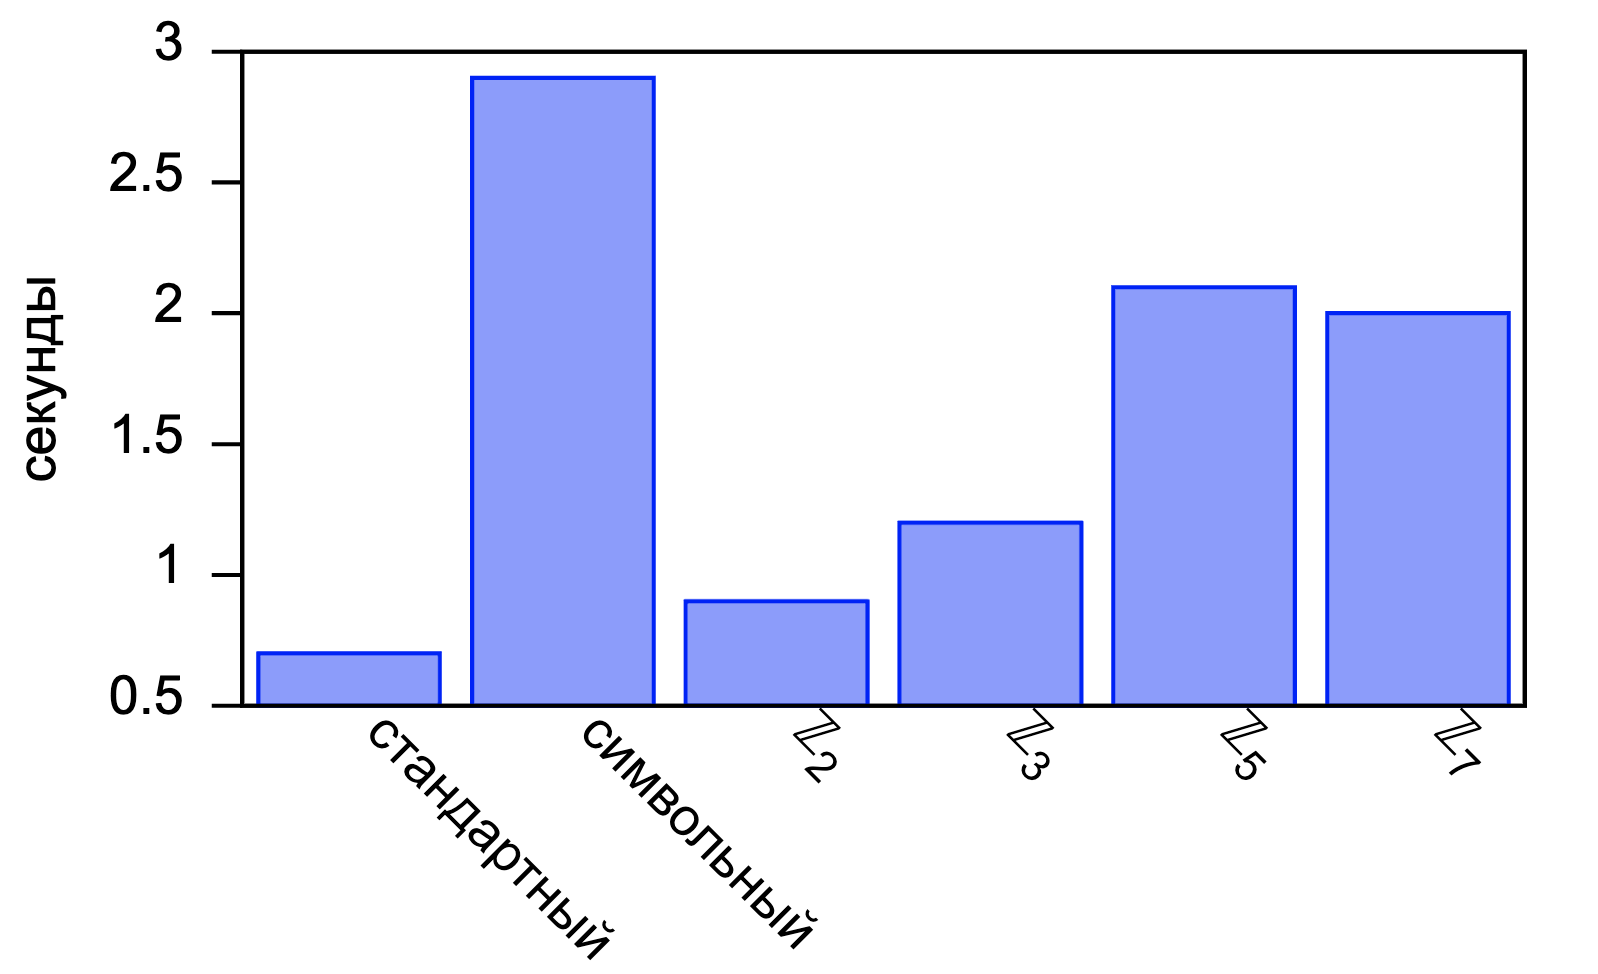
\includegraphics[width=0.85\linewidth]{../gnuplot/single/det/plot.png}}
\caption{График производительности однопоточных методов для вычисления определителя матрицы.}
\label{img:single:det:1}
\end{figure}

\begin{figure}[H]
\centerline{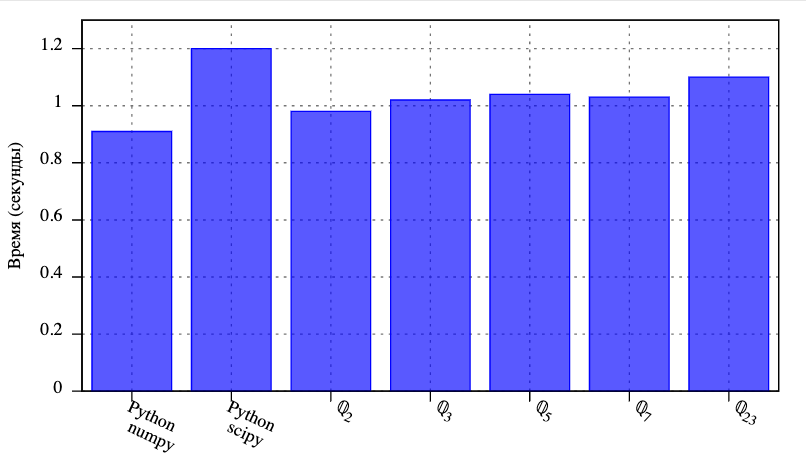
\includegraphics[width=0.85\linewidth]{../gnuplot/single/det/wosymb.png}}
\caption{График производительности однопоточных методов для вычисления определителя матрицы (без символьного метода).}
\label{img:single:det:2}
\end{figure}

Как видно из результатов обычные методы из пакета |numpy| работают немного быстрее, чем $p$-адические методы, а методы из пакета |scipy| работают сопоставимое с $p$-адическими методами время. Для наглядности, на графике \ref{img:single:det:2} видно, что символьные методы работают в разы дольше чем классические и $p$-адические методы.

\subsubsection{Решение СЛАУ}
Для сравнения производительности классического и $p$-адического метода решения СЛАУ решим $m$ раз систему из $n$ уравнений:

\begin{equation}
\boldsymbol{A}*\boldsymbol{X}=\boldsymbol{B},
\end{equation}

\noindent где $\boldsymbol{A}$ - матрица коэффициентов размером $n \times n$, $\boldsymbol{X}$ - вектор неизвестных и $\boldsymbol{B}$ - вектор правых частей.
Пусть коэффициенты матрицы $\boldsymbol{A}$ вычисляются следующим образом:

\begin{equation}
a_{i,j}= 
\begin{cases} 
\abs{1-rand(n)*round\bigg(i-j\bigg)^2}, i \neq j, \\ 
10, i = j,
\end{cases}
\end{equation}

\noindent где |rand(n)| некоторое случайное число в диапазоне от $0$ до $n$. При этом получается положительно определенная матрица. Например, для $n=5$ матрица $\boldsymbol{A}$ будет иметь вид:

$$
\begin{pmatrix}
  10 & 7 & 23 & 53 & 79 \\
  0 & 10 & 8 & 11 & 80 \\
  35 & 2 & 10 & 7 & 11 \\
  17 & 3 & 7 & 10 & 1 \\
  72 & 63 & 11 & 1 & 10
\end{pmatrix}.
$$

Пусть на каждом шаге решения $k=1 \dots m$ коэффициенты вектора правых частей равны номеру шага: $b_i = k$.
Чтобы контролировать правильность решения каждым программным средством будем подсчитывать сумму коэффициентов вектора $\boldsymbol{X}$ на каждом шаге решения и суммировать ее по шагам:

\begin{equation}
S = \sum\limits_{k=1}^{m}\sum\limits_{i=1}^{n} x_i^{(k)}.
\end{equation}

Тестировать будем два метода решения СЛАУ - метод Гаусса и метод Крамера. Оба метода будем тестировать при размере матрицы $n=1000$ и числе повторений $m=100$ шагов. Договоримся, что разложение (факторизацию) матрицы $\boldsymbol{A}$ будем делать на каждом шаге, это значит, что каждый раз систему уравнений будем решать полностью. Время решения будем измерять по циклу решения СЛАУ – без учета предварительной подготовки матрицы $\boldsymbol{A}$.

Разные запуски реализаций решения на ПК дают несколько разное время поскольку ОС периодически отбирает ресурсы от запущенной программы для своих нужд. Из нескольких запусков будем записывать минимальное время.

Будем, для наглядности, так же сравнивать различные числа из таких полей как $\mathbb{Q}_2$, $\mathbb{Q}_3$, $\mathbb{Q}_5$, $\mathbb{Q}_7, \mathbb{Q}_{23}$.
 
\begin{figure}[H]
\centerline{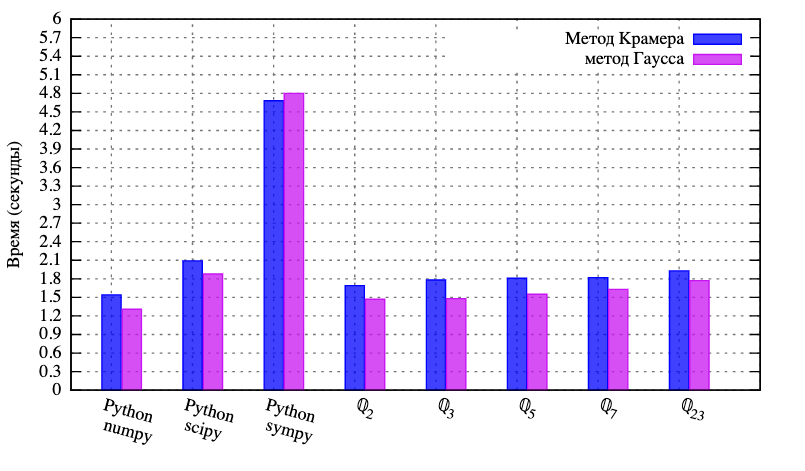
\includegraphics[width=0.85\linewidth]{../gnuplot/single/system/plot.png}}
\caption{Сравнение производительности однопоточных методов для решения СЛАУ.}
\label{img:single:system:1}
\end{figure}
 
\begin{figure}[H]
\centerline{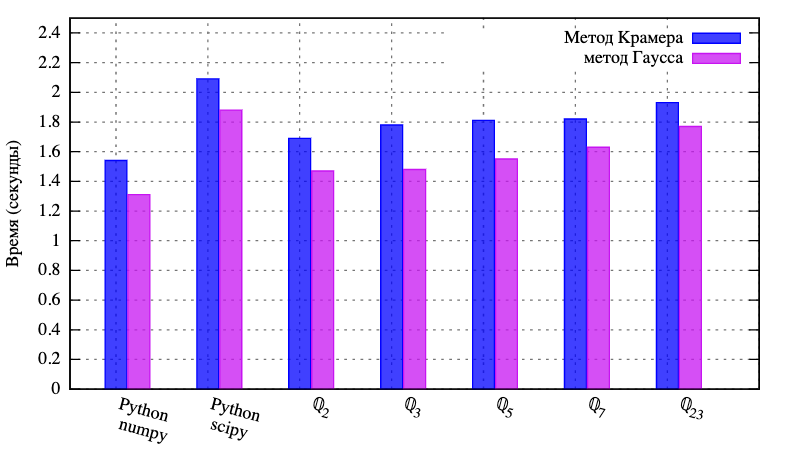
\includegraphics[width=0.85\linewidth]{../gnuplot/single/system/wosymb.png}}
\caption{Сравнение производительности однопоточных методов для решения СЛАУ (без символьного метода).}
\label{img:single:system:2}
\end{figure}
 
 
Полученные результаты производительности сопоставимы с результатами полученными для вычисления определителя матрицы и так же как и там методы из пакета |numpy| работают немного быстрее $p$-адических методов, а методы из пакета |sympy| немного дольше. Кроме того видно, что метод Гаусса работает быстрее, что является очевидным фактом, так как его алгоритмическая сложность ниже, чем у метода Крамера.
 
 %-------------------------------------------------------------------%
\section{Разработка многопоточной библиотеки для работы с $p$-адической арифметикой}

\subsection{Описание многопоточной $p$-адической арифметики}

Многопоточный алгоритм для $p$-адических чисел впервые был предложен Моррисоном \cite{bib:numbers:morrison}. Алгоритм основан на китайской теореме об остатках, которая расширена на случай использования рациональных чисел. Процесс декодирования $p$-адической последовательности в этом случае выглядит следующим образом: если $r \sim \{r_1,r_2,\cdots, r_s\}$ является представлением остатка рационального числа $a$ по модулям $\{r_1,r_2,\cdots, r_s\}$, где наибольший общий делитель $GCD(p_i, p_j) =1 \; \forall i \neq j$, то тогда процесс декодирования осуществляется с помощью алгоритма \ref{algo:decoding}\cite{bib:numbers:newman}\cite{bib:numbers:dixon}.


\begin{algorithm}
\DontPrintSemicolon % Some LaTeX compilers require you to use \dontprintsemicolon instead
\Begin {
	$p$ := $\prod\limits_{i=1}^{s} p_i $ \\
	\For{$i \gets 1$ \textbf{to} $s$} {
		найти $p_{i}^{'}: \frac{p}{p_i}p_{i}^{'} \equiv 1 \pmod {p_i}$
	}
	$\overline{r}=\sum\limits_{i=1}^{s} p_{i}^{'}r_i \pmod p$
	
	
	$u_{-1}=p, u_0=\overline{r}$ \\
	$v_{-1}=0, v_0=1$ \\
	$i=-1$ \\
	\While{$u_i \textless \sqrt{p}$} {
		$q_i=\lfloor{\frac{u_{i-1}}{u_i}}\rfloor$ \\
		$u_{i+1}=u_{i-1}-q_i u_i$ \\
		$v_{i+1}=v_{i-1}+q_i v_i$ \\
		$i = i +1$
	}
	
	
	\Return $r=((-1)^{i} \frac{u_i}{v_i})$
}
\caption{декодирование $p$-адического числа.}
\label{algo:decoding}
\end{algorithm}

Комбинируя $p$-адическую арифметику и китайскую теорему об остатках получается многопоточный алгоритм для $p$-адической арифметики представленный в виде блок-схемы на рисунке \ref{img:multi:schema}.

\begin{figure}[H]
\centerline{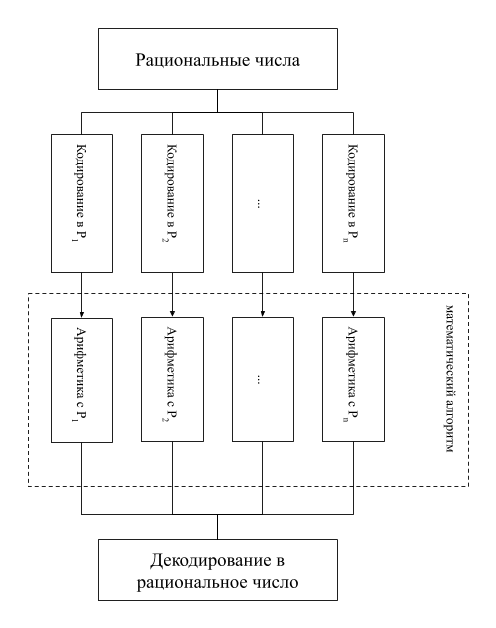
\includegraphics[width=0.7\linewidth]{images/multi/schema.png}}
\caption{Китайская теорема об остатках, скомбинированная с $p$-адической арифметикой.}
\label{img:multi:schema}
\end{figure}

Далее, рассмотрим метод для определения наличия или отсутствия переполнения. Для начала необходимо ввести определение переполнения.

\begin{defn}
Рациональное число $\frac{a}{b} \pmod{p_i}$, которое определяет последовательность $r \sim \{r_1,\cdots, r_s\}$ при условии, что $\gcd{(a, b)}=1$ не может быть однозначно восстановлено с помощью обратного преобразования \ref{th:backward_mapping} для  алгоритмов, которые основаны на китайской теореме об остатках примененной для простых чисел $\{p_1,\cdots, p_s\}$. Данная ситуация называется переполнением.
\end{defn}

Один из методов для обнаружения переполнения это предсказывание верхней границы вычислений, а затем определение размера простого множества $\{p_1,p_2, \cdots, p_n\}$ как это сделано в \cite{bib:numbers:matula}. Другой способ для определения переполнения - использование дополнительных цифр в последовательности $p$-адического числа, как это сделано в \cite{bib:numbers:hensel:overflow}. Этот метод может определять переполнение на основе набора простых чисел $\{p_1,\cdots, p_n\}$ и вычисления остаточного набора чисел. В этом методе каждая числовая последовательность должна иметь дополнительные числа, используемые для сохранения последовательности состоящей из $k$ чисел.
С помощью набора простых чисел $\{p_1,p_2, \cdots, p_i, p_{i+1}, \cdots, p_{i+k}\}$ для любого рационального числа $x$ получается последовательность $\{r_1 = x \pmod{p_1},\cdots, r_{i+k}= x\pmod{p_{i+k}}\}$, запишем ее как $x \sim \{r_1, r_2, \cdots, r_{i}, r_{i+1}, \cdots, r_{i+k}\}$.
Во время процесса определения наличия переполнения это будет рассматриваться как

\begin{equation}
x \sim (r_0, r_1, \cdots, r_i, r_{i+1}, \cdots, r_{i+k}),
\end{equation}

\noindent где $ r_{i+1}, \cdots, r_{i+k}$ является проверочной частью последовательности.

Теперь можно ввести критерий существования или отсутствия переполнения, который используется в программной реализации $p$-адической арифметики.

\begin{defn}
Переполнение для последовательности $x$ случится, если 	

\begin{equation}
Decoding(x,i) \neq Decoding(x,i+k).
\end{equation}

\noindent и не случится, если

\begin{equation}
Decoding(x,i) = Decoding(x,i+k). 
\end{equation}
\end{defn}

\subsection{Многопоточный метод решения СЛАУ}
Стандартная схема вычисления вектора решения $\boldsymbol{x}$ для СЛАУ $\boldsymbol{A}\cdot \boldsymbol{x} = b$ содержит представление рациональных чисел с помощью $p$-адических чисел в виде кода Гензеля и выполнении операций над данными числами. Однако, как видно из теоремы \ref{th:backward_mapping} представление чисел в виде кода Гензеля возможно только когда ожидаемый результат будет принадлежать множеству $\mathbb{F}_{p,r}$. Это значит, что неоходимо  произвести правильный выбор чисел $p$ и $r$.


Перед тем как переходить к описанию параллельного метода решения СЛАУ необходимо представить последовательный метод Гаусса.

\begin{problem}
Пусть дана матрица $\boldsymbol{A} \in \mathbb{Q}^{n \times n}$ вектор $\boldsymbol{b} \in \mathbb{Q}^{n}$. Найти вектор $\boldsymbol{x}=(x_1,\cdots,x_n) \in \mathbb{Q}^{n}$ такой, что:

\begin{equation}
\boldsymbol{A}\cdot \boldsymbol{x} = b.
\end{equation}

\end{problem}

Для начала предположим, что $\boldsymbol{A} \in \mathbb{Z}^{n \times n}$ и $\boldsymbol{b} \in \mathbb{Z}^{n}$. Используя правило Крамера мы знаем, что 

\begin{equation}\label{formula:kramer}
x_i=\frac{\Delta_i}{\Delta_i},	
\end{equation}

\noindent где $\Delta$ это определитель матрицы $A$, а $\Delta_i$ это определитель, получаемый из определителя $\Delta$ путем замены $i$-го столбца на столбец свободных членов. Известно, что если взять для любой матрицы $\mathbb{Z}^{n \times n}$ число $a$, которое будет максимальным среди остальных элементов, то оно будет удоволетворять неравенству

\begin{equation}
\mid M \mid \leq n!a^n.
\end{equation}

\noindent Из этого выражения и формулы \ref{formula:kramer} получим, что числитель и знаменатель для любого $x_i$ ограничен числом $n!a^n$, где $a$ максимальное значение матрицы $A$. Из этого ограничения можно определить число $r \in \mathbb{F}_{p,r}$ для данного простого числа $p$. Из определения достаточно того, что

\begin{equation}\label{formula:det:1}
n!a^b \leq \sqrt{\frac{p^r-1}{2}}.
\end{equation}

Принимая во внимание квадрат в левой стороне неравенства мы получаем, что 

\begin{equation}
2{(n!a^n)}^2+1\leq p^r.
\end{equation}

\noindent Неравенство в свою очередь аналогично следующему:

\begin{equation} \label{eq:matrix:r}
r \geq log_p(2{(n!a^n)}^2+1).
\end{equation}

Известно, что неравенство Адамара рассмотренное в например \cite{bib:numbers:mignotte} и \cite{bib:numbers:marcus} представляет следующее ограничение для определителя:

\begin{equation}
{\mid A \mid}^2 \leq \prod\limits_{i=1}^{n}{\bigg(\sum\limits_{j=1}^{n} a^2_{i,j} \bigg)}^{\frac{1}{2}}
\end{equation}

\noindent Из этого неравенства и неравенства \ref{formula:det:1} следует условие:

\begin{equation}
p^r \leq \sum\limits_{i=1}^{n} {\mid b_i \mid} \prod\limits_{i=1}^{n}{\bigg(\sum\limits_{j=1}^{n} a^2_{i,j} \bigg)}^{\frac{1}{2}}.
\end{equation}

Должно быть отмечено, что оба ограничения являются строгими и меньший выбор чисел $p$ и $r$ частно достаточен. В обычном случае $A \in \mathbb{Q}^{n \times n}$ и и $\boldsymbol{b} \in \mathbb{Q}^{n}$ ограничением для числителя и знаменателя для числа $x_i$ становится $n!a^{n(n+1)}$. 

\begin{thethm}
Пусть $n_1,n_2,\dots, n_k$ - натуральные попарно взаимно простые числа, а $r_1,r_2,\dots,r_k$ - некоторые целые числа, тогда существует такое целое число $M$, что оно будет решением системы сравнений:

\begin{equation}
\begin{cases} 
M \equiv r_1 \pmod {n_1}, \\
M \equiv r_2 \pmod {n_2}, \\
\dots \\
M \equiv r_k \pmod {n_k}.
\end{cases}
\end{equation}

\noindent При этом для любых двух решений $A$ и $B$ этой системы справедливо

\begin{equation}
A \equiv B \pmod {n_1,n_2,\dots,n_k},
\end{equation}

\noindent то есть решение системы сравнений существует и единственно по модулю $n_1,n_2,\dots,n_k$.
\end{thethm}


Будем описывать параллельный алгоритм для решения СЛАУ для $k$ процессов (или независимых потоков). Для начала нужно вычислить $k$ простых чисел $p_1, \dots, p_k$ случайным образом, которые удовлетворяют длинне кода $r$ так, что числа из вектора $x$ содержатся в $\mathbb{F}_{g,r}$, где $g=p_1,\dots,p_k$. 
Запустим $k$ параллельных задач. Каждая из них вычисляет образ в отношении одного простого числа в представлении рациональных элементов, т.е. $H_{p_i,r}(A)$ и $H_{p_i,r}(b)$.
После, каждый процесс запускает метод Гаусса. \\

\begin{algorithm}
\DontPrintSemicolon % Some LaTeX compilers require you to use \dontprintsemicolon instead

\KwIn{ $n$: степень системы \newline
       $A=(a_{i,j}) \in \mathbb{Q}^{n \times n}$: квадратная, $\dim(A)=n \times n$ \newline
       $b=(a_{1,n+1},\dots,a_{n,n+1}) \in \mathbb{Q}^{n}$: $\dim(b)=n$ \newline
       $p$: простое число }

\KwOut{$x=(x_1,\dots,x_n) \in \mathbb{Q}^{n}$: решение $Ax = b$ если существует.}

\Begin {
Найти максимум $a$ среди числителей и знаменателей среди чисел входящих в состав $A$ и $b$.

Вычислить порядок числа $r$ по формуле \ref{eq:matrix:r}.

Преобразовать числа входящие из $A$ и $b$ в код Гензеля $H_{p,r}$.

l := 0\;
\For{$i \gets 1$ \textbf{to} $n$} {
  l := l + 1 \;
  \For{$j \gets 1$ \textbf{to} $n+1$} {
      Поделить $a_{i,j}$ на $a_{i,i}$.
  }
   \For{$h \gets l+1$ \textbf{to} $n$} {
      Умножить $i$-ю строку на $a_{h,l}$\;
      Вычесть полученную $i$-ю строку на $h$-ю строку системы полученную последней операцией. Это новая $h$-я строка.
  } 
}

Восстановить $H_{p,r}(x_1), \cdots, H_{p,r}(x_n)$ из полученной треугольной матрицы.
}


\caption{Алгоритм Гаусса для $p$-адической арифметики.}
\label{algo:gauss}
\end{algorithm}


Представленный алгоритм \ref{algo:gauss} вычисляет решения $x^{(i)} \in \mathbb{H}_{p_i,r}^n$ для $i = \overline{1,k}$. После получения всех $x^{(i)}$ выполняется $k$ параллельных запусков алгоритма расширенной китайской теоремы об остатках. Будем применять параллельную версию расширенного алгоритма китайской теоремы об остатках описанную в \cite{bib:numbers:limongelli} для каждой последовательности компонентов $x_j^{(1)}, \dots, x_j^{(k)}$, получая компоненты $x_j \in \mathbb{H}_{p_1,\dots,p_k,r}$ вектора решения $x$.
Из предположений сделанных для числа $r$, полученный список результатов $\{x^{(1)},\dots,x^{(k)}\}$ может быть преобразован обратно в вектор $x \in \mathbb{F}_{g,r}^n$ с помощью китайской теоремы об остатках. Из теоремы \ref{th:hensel} известно, что если решение существует в $\mathbb{F}_{g,r}$, то оно уникальное.
После этого, результат $x$ должен быть сконвертирован из $p$-адического представление, в обычное с помощью теоремы \ref{th:backward_mapping}, применимой параллельно к каждому из компонентов. Схема параллельных вычислений представлена ниже на рисунке \ref{img:multi:gauss}.

\begin{figure}[H]
\centerline{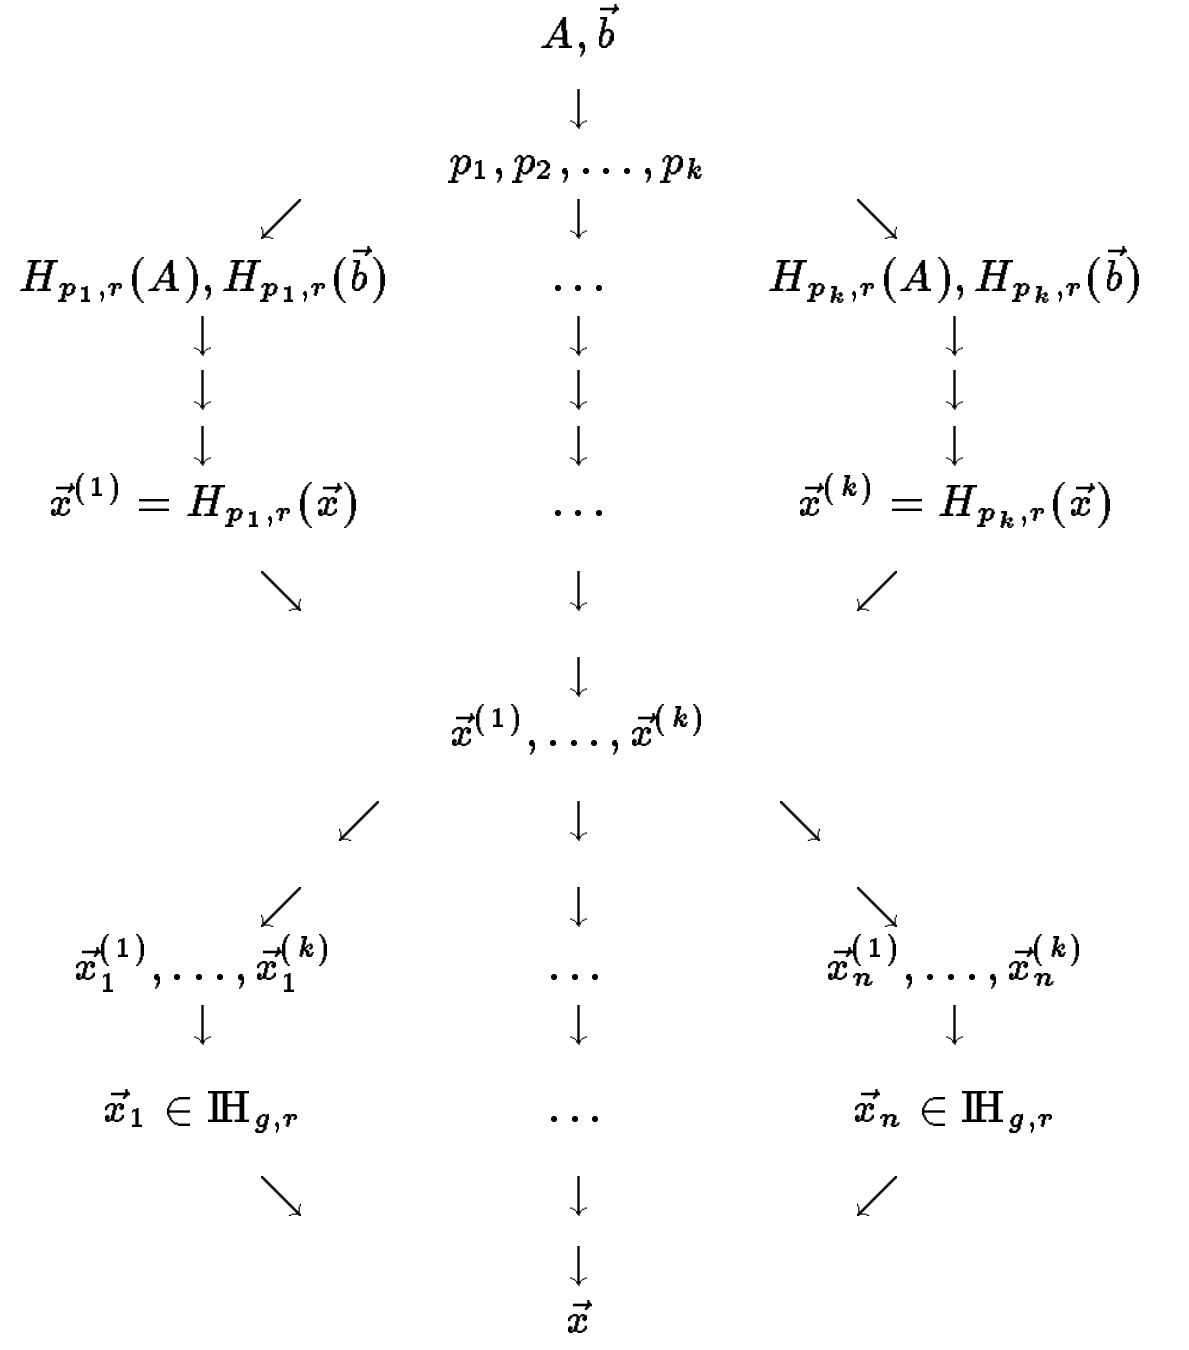
\includegraphics[width=0.7\linewidth]{images/multi/native.png}}
\caption{Схема параллельного алгоритма для нахождения решения СЛАУ методом Гаусса.}
\label{img:multi:gauss}
\end{figure}


В случае с матрицами очень больших размерностей, в разы больших, чем количество доступных процессоров, могут быть использованы стандартные методы для распараллеливания матричных операций.


\subsection{Многопоточный метод для вычисления собственных значений и собственных векторов}

Нахождение собственных значений и собственных векторов матриц - одна тех сложных вычислительных задач, с которой часто приходится сталкиваться специалисту, занимающемуся проектированием или анализом больших технических систем.  В электрических и механических системах собственные числа отвечают собственным частотам колебаний, а собственные векторы характеризуют соответствующие формы колебаний. В теории динамических систем и связанных с ними системах линейных дифференциальных уравнений, знание собственных значений позволяет определить характер поведения системы во времени и решить вопрос об устойчивости такой системы. Оценка величин критических нагрузок при расчете строительных конструкций также основана на информации о собственных значения и собственных вектора матриц. 

Одним из методов нахождения нахождения собственных векторов и собственных значений является метод Якоби или как его еще называют метод вращений. Метод Якоби был предложен Карлом Густавом Якоби в 1846 году и представляет собой итерационный алгоритм вычисления собственных значений и собственных векторов симметричной матрицы. Метод основан на построении последовательности матриц, которые ортогонально подобны исходной матрице и имеют монотонно убывающие до нуля суммы всех внедиагональных элементов. Данный метод так же без существенных изменений метод вращений переносится на эрмитовы и косоэрмитовы матрицы. В данной работе будет рассматривать только метод, где матрица $A$ является вещественной и симметричной. Алгоритмы для случая комплексной эрмитовой матрицы можно посмотреть в \cite{bib:numbers:voevodin}.

Прежде чем переходить к описанию алгоритма и рассмотрению его особенностей связанных с применением $p$-адической арифметики необходимо ввести несколько определений.


\begin{defn}
Число $\lambda$ называется собственным значением матрицы $A$, если существует такой ненулевой вектор $x=(x_1,x_2,\cdots,x_n)$ удоволетворяющий уравнению

\begin{equation}
Ax=\lambda x
\end{equation}
	
\noindent и называемый собственным вектором матрицы $A$, отвечающим собственному значению $\lambda$.
\end{defn}


\begin{defn}
Матрицей вращения или матрицей поворота называется ортогональная матрица, которая используется для выполнения собственного ортогонального преобразования в евклидовом пространстве. При умножении любого вектора на матрицу поворота длина вектора сохраняется. Определитель матрицы поворота равен единице.
\end{defn}

Будем описывать параллельный алгоритм для нахождения собственных значений и собственных векторов матрицы $A$ для $k$ процессов (или независимых потоков). Для начала нужно вычислить $k$ простых чисел $p_1, \dots, p_k$ случайным образом, которые удовлетворяют длинне кода $r$ так, что числа из вектора $x$ содержатся в $\mathbb{F}_{g,r}$, где $g=p_1,\dots,p_k$. 
Запустим $k$ параллельных задач. Каждая из них вычисляет образ в отношении одного простого числа в представлении рациональных элементов, т.е. $H_{p_i,r}(A)$ и $H_{p_i,r}(b)$. После этого выполняется последовательный метод Якоби.

Алгоритм \ref{algo:jacoby} вычисляет значения $\lambda_i$ и $x_i$ для матрцы $A$. После получения всех собственных векторов и всех собственных чисел выполняется $k$ параллельных запусков китайской теоремы об остатках. Будем применять параллельную версию китайской теоремы об остатках описанную в \cite{bib:numbers:limongelli} для каждой последовательности компонентов $x_j^{(1)}, \dots, x_j^{(k)}$ и $\lambda_j^{(1)}, \dots, \lambda_j^{(k)}$, получая компоненты $x_j \in \mathbb{H}_{p_1,\dots,p_k,r}$ и $\lambda_j \in \mathbb{H}_{p_1,\dots,p_k,r}$. Вспомогательные функции |maxind|, |rotate| и |update| для алгоритма \ref{algo:jacoby} приведены в приложении \ref{appendix:2}.

Полученный список результатов $\{x^{(1)},\dots,x^{(k)}\}$ может быть преобразован обратно в вектор $x \in \mathbb{F}_{g,r}^n$ с помощью китайской теоремы об остатках.

После этого, результа должен быть сконвертирован из $p$-адического представления, в обычное с помощью теоремы \ref{th:backward_mapping}, применимой параллельно к каждому из компонентов.

\begin{algorithm}
\DontPrintSemicolon % Some LaTeX compilers require you to use \dontprintsemicolon instead

\KwIn{ $n$: степень системы \newline
       $A=(a_{i,j}) \in \mathbb{Q}^{n \times n}$: симметричная, $\dim(A)=n \times n$ \newline
       $p$: простое число }

\KwOut{ $\lambda$: вектор содержащий все собственные значения матрицы $A$ \newline
        $x$: список содержащий все собственные вектора матрицы $A$ }

\Begin {
Найти максимум $a$ среди числителей и знаменателей среди чисел входящих в состав $A$.

Вычислить порядок числа $r$ по формуле \ref{eq:matrix:r}.

Преобразовать числа входящие из $A$ в код Гензеля $H_{p,r}$.

Инициализацировать $e, E$ и массивы $ind, changed$.

$E := I; \; state := n;$

\For{$k \gets 1$ \textbf{to} $n$} {
	$ind_k := maxind(k); \; e_k := S_{kk}; \; changed_k$ := true 
}

\While{$state \neq 0$} {
	$m := 1$
	
	%! find index (k,l) of pivot p
	\For{$k \gets 2$ \textbf{to} $n-1$} {
		\lIf{ \abs{S_{k,ind_{k}}} > \abs{S_{m,ind_{m}}} } {
			$m := k$
		}
	}
	$k := m; \; l := ind_m; \; p := S_{kl};$
	
	$c = \cos(\phi); \; s = \sin(\phi);$
	
    $y := (e_l-e_k)/2; \; d := \mid y \mid +\sqrt{p_2+y_2};$
    
    $r := \sqrt{p_2+d_2}; c := d/r; \; s := p/r; t := p_2/d;$
   	
   	\lIf{ y < 0 } {
		$s := -s; t := -t$
	}
	
	$S_kl := 0;$ 
	
	$update(k,-t); \; update(l,t)$
	
	%! rotate rows and columns k and l
	\lFor{$i \gets 1$ \textbf{to} $k-1$} {
		$rotate(i,k,i,l)$
	}
	\lFor{$i \gets k+1$ \textbf{to} $l-1$} {
		$rotate(k,i,i,l)$
	}
	\lFor{$i \gets l+1$ \textbf{to} $n$} {
		$rotate(k,i,l,i)$
	}
	%! rotate eigenvectors
	
	\lFor{$i \gets 1$ \textbf{to} $n$} {
	$$
	\begin{pmatrix}
	  E_{ik} 
	  E_{il} 
	\end{pmatrix}
	:=
	\begin{pmatrix}
	  c & -s \\
	  s & c
	\end{pmatrix}
	\cdot
	\begin{pmatrix}
	  E_{ik} 
	  E_{il} 
	\end{pmatrix}
	$$
	}
	%! rows k, l have changed, update rows indk, indl
    $ind_k := maxind(k); \; ind_l := maxind(l);$
}
}
Восстановить $H_{p,r}(x_1), \cdots, H_{p,r}(x_n)$ и $H_{p,r}(\lambda_1), \cdots, H_{\lambda,r}(\lambda_n)$.
\caption{Алгоритм Якоби для $p$-адической арифметики.}
\label{algo:jacoby}
\end{algorithm}



%-------------------------------------------------------------------%
\section{Сравнение производительности классических и $p$-адических методов на примере прикладных задач}

Для точного сравнения производительности методов все тесты будут производятся на компьютере с процессором Intel Core i5-7360U и 16 Гб оперативной памяти. Для тестов будем использовать 4 параллельных потока.

\subsection{Решение СЛАУ}
Подход к тестированию нахождения решения СЛАУ будет производится тем же методом, что и в случае однопоточных $p$-адических методов. Сравнение будет производиться между символьным методом решения СЛАУ из пакета |scipy|, с методом для решения СЛАУ из пакета |numpy|, а так же с однопоточным и многопоточным $p$-адическим методом Гаусса. Для наглядности тесты будут произведены для $p$-адических чисел из $\mathbb{Q}_2$, $\mathbb{Q}_3$, $\mathbb{Q}_5$, $\mathbb{Q}_7, \mathbb{Q}_23$. 


\begin{figure}[H]
\centerline{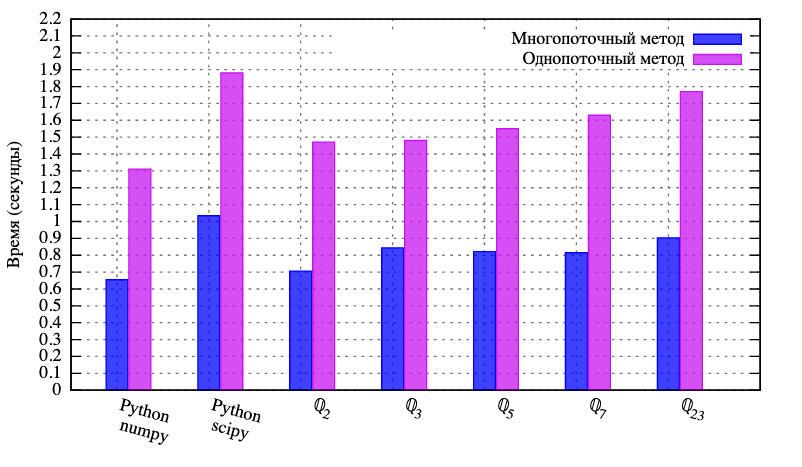
\includegraphics[width=0.85\linewidth]{../gnuplot/multi/gauss/plot.png}}
\caption{Сравнение методов для решения СЛАУ}
\label{img:multi:gauss}
\end{figure}

На рисунке \ref{img:multi:gauss} приведено сравнение, где видно, что многопоточные $p$-адические методы не уступают традиционным методам из популярных библиотек для ЯП Python, а в некоторых случаях даже превосходят. Так же видна разница между многопоточными и однопоточными методами - результат времени вычисления различается в несколько раз, из чего можно сделать вывод, что параллелизация очень важна при работе с $p$-адическими числами и методами, которые оперируют над ними.

\subsection{Вычисление собственных значений и собственных векторов}
Сравнение вычисления собственных значений и собственных векторов симметричной матрицы $A$ будем производить с помощью итерационного метода Якоби называемого методом вращений, который основан на приведении матрицы $A$ к диагональному виду.

Идея метода Якоби состоит в том, чтобы обнулять недиагональные элементы вращениями до тех пор, пока они все не обнулятся и получится диагональная матрица. После каждого вращения сумма квадратов внедиагональных элементов уменьшается, что приводит к сходимости процесса диагональности. Алгоритм и более подробное описание метода Якоби приведено в предыдущем разделе.

Тесты будем производить на матрице размера $1000 \times 1000$, каждое вычисление будем производить $100$ раз. 

\begin{figure}[H]
\centerline{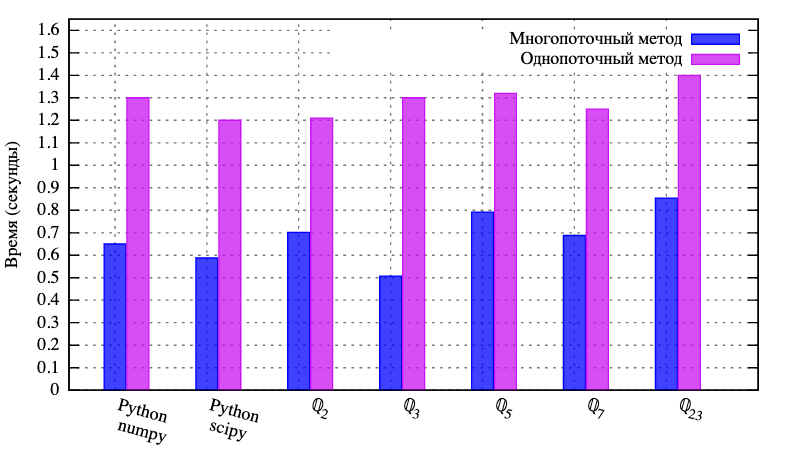
\includegraphics[width=0.85\linewidth]{../gnuplot/multi/jacoby/plot.png}}
\caption{Сравнение методов для нахождения собственных чисел и собственных векторов матрицы.}
\label{img:multi:jacoby}
\end{figure}

Из представленного графика \ref{img:multi:jacoby} видно, что как и в случае с нахождением решения СЛАУ многопоточные $p$-адические методы нахождения собственных чисел и векторов не уступают, а в некоторых случаях являются более быстрыми, по сравнению с методами из стандартных библиотек ЯП Python. Также видно, что разная база для $p$-адических чисел дает немного различный результат и оптимальной базой является $p=2$ или $p=3$.

\subsection{Решение ОДУ}
Для сравнения времени решения обыкновенных дифференциальных уравнений возьмем простейшее дифференциальное уравнение падающей \mbox{сферы:}

\begin{equation}
\begin{aligned}
\dfrac{\partial z}{ \partial t} = v, \\
\dfrac{\partial v}{ \partial t} = g - \alpha v^2, \\
\alpha = \frac{3\rho_f}{4\rho_k d}C_d.
\end{aligned}
\end{equation}

\noindent Аналитическое решение данного уравнения при $z(0)=0$ и $v(0)=0$ представляет собой следующие функции:

\begin{equation}
\begin{aligned}
z(t)=\frac{\log{(\cosh{(\sqrt{\alpha g} \cdot t})})}{\alpha}, \\
v(t)=\sqrt{\frac{g}{\alpha}} \cdot \tanh{(\sqrt{\alpha g} \cdot t)}
\end{aligned}
\end{equation}

\noindent Конечная скорость $v_t$ находится из уравнения $\frac{\partial v}{ \partial t}$ и равна $v_t=\sqrt{\frac{g}{\alpha}}$.

В качестве физических параметров для эксперимента будем использовать параметры стандартного мяча для гольфа:

\begin{threeparttable}
\begin{longtable}[H]{lp{0.7\linewidth}}
{$d$} -- диаметр шара & 41 [мм] \\
{$\rho_k$} -- плотность сферы & 1275 [кг/м\textsuperscript{3}] \\
{$\rho_f$} -- плотность жидкости & 1.22 [кг/м\textsuperscript{3}] \\
{$C_d$} -- коэффициент трения & 0.4 
\end{longtable} 
\end{threeparttable}


При этих параметрах $\alpha$=$7 \cdot 10^{-3}$, а конечная скорость становится равной $v_t=\sqrt{\frac{g}{\alpha}}=37.44$.

Для сравнения методов будем использовать стандартную схему метода Рунге-Кутты 4-го порядка:

\begin{equation}%\label{eq:task:2}
\begin{aligned}
k_1 = f(x_n, y_n), \\
k_2 = f(x_n+\frac{h}{2}, y_n+\frac{h}{2}k_1), \\
k_3 = f(x_n+\frac{h}{2}, y_n+\frac{h}{2}k_2), \\ 
k_4 = f(x_n+h, y_n+hk_3), \\
y_{n+1}=y_n+\frac{h}{6}(k_1+2k_2+2k3+k_4).
\end{aligned}
\end{equation}


\noindent И схему метода Эйлера:

\begin{equation}%\label{eq:task:2}
\begin{aligned}
y_{n+1}=y_n+h \cdot f(x_n, y_n).
\end{aligned}
\end{equation}


Разные запуски реализаций решения на ПК дают несколько разное время поскольку ОС периодически отбирает ресурсы от запущенной программы для своих нужд. Из нескольких запусков будем записывать минимальное время. Запускать тесты будем $100$ раз. Из нескольких запусков будем записывать минимальное время.

Для наглядности будем сравнивать время нахождения решения ОДУ между классическими методами из таких стандартных библиотек ЯП Python как |numpy| и |scipy| и $p$-адическими методами, которые используют числа из $\mathbb{Q}_2$, $\mathbb{Q}_3$, $\mathbb{Q}_5, \mathbb{Q}_5$ и $\mathbb{Q}_{23}$.

\begin{figure}[H]
\centerline{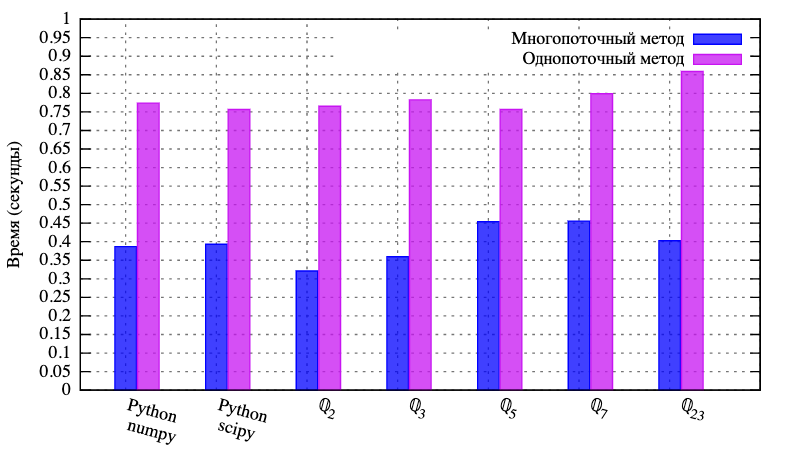
\includegraphics[width=0.85\linewidth]{../gnuplot/multi/euler/plot.png}}
\caption{Сравнение методов для нахождения численного решения ОДУ с помощью метода Эйлера.}
\label{img:multi:ode:euler}
\end{figure}


Как видно из представленного графика \ref{img:multi:ode:euler} - метод Эйлера дает неплохие результаты с использованием параллельной $p$-адической арифметики.


\begin{figure}[H]
\centerline{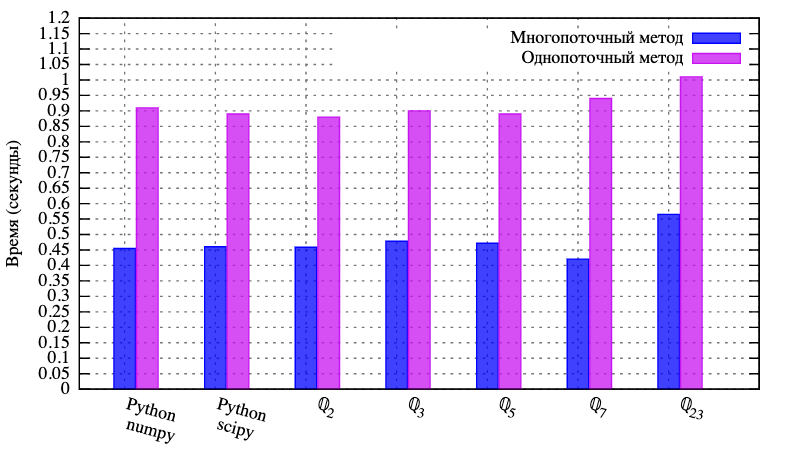
\includegraphics[width=0.85\linewidth]{../gnuplot/multi/rk/plot.png}}
\caption{Сравнение методов для нахождения решения ОДУ с помощью метода Рунге-Кутты 4-го порядка.}
\label{img:comp:ode:rk}
\end{figure}

\begin{figure}[H]
\centerline{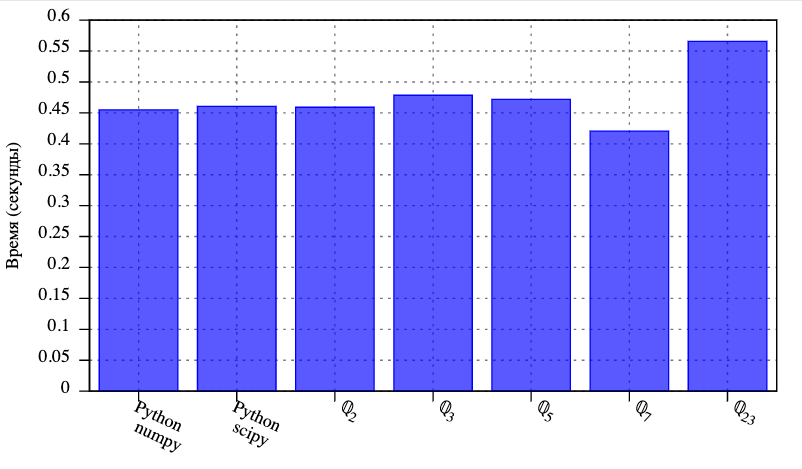
\includegraphics[width=0.85\linewidth]{../gnuplot/multi/rk/multi.png}}
\caption{Сравнение классических методов для нахождения решения ОДУ с помощью метода Рунге-Кутты 4-го порядка и методов с использованием параллельной $p$-адической арифметики.}
\label{img:comp:ode:rk:multi}
\end{figure}

Как видно из представленных графиков \ref{img:comp:ode:rk}, \ref{img:comp:ode:rk:multi} - метод Рунге-Кутты 4-го порядка с помощью использования $p$-адической арифметики работает даже лучше, чем классические методы представленные в стандартных библиотеках в случае использования многопоточных методов. В случае использования однопоточного метода $p$-адический метод дает сопоставимое с классическим методом время решения.

\subsection{Вычисление $e^{Ax}$}

Матричная экспонента возникает при многих задачах связанных с механикой и вычислительной техникой, в частности очень часто матричную экспоненту можно встретить в рассмотрении задачи Коши для линейной системы обыкновенных дифференциальных уравнений с постоянными коэффициентами. Иногда такие системы возникают после частичной дискретизации уравнений в частных производных, например, в методах конечных элементов. Тогда матрица $A$ является некоторой конечномерной аппроксимацией дифференциального оператора. Как следствие, число строк матрицы $A$ может легко достигать тысяч, миллионов и даже нескольких миллиардов. Такие матрицы даже невозможно хранить в виде квадратного массива, поэтому их хранят в специальных разреженных форматах представления.

Перед тем как переходить к вычислению экспоненты и сравнению результатов введем ряд определений, необходимых для описания алгоритма который использует полиномиальный метод и на основании которого будет производится сравнение классических и $p$-адических алгоритмов вычисления $e^{At}$.

\begin{defn}\label{def:exp}
Экспонентой от матрицы $A$ называется матрица

\begin{equation}
e^A=I+A+\frac{1}{2!}A^2+\cdots++\frac{1}{n!}A^n + \cdots,
\end{equation}

\noindent соответственно

\begin{equation}
e^{At}=I+tA+\frac{t^2}{2!}A^2+\cdots++\frac{t^n}{n!}A^n + \cdots.
\end{equation}
\end{defn}

Надо отметить, что представленное определение \ref{def:exp} не требует никаких дополнительных конструкций, кроме сложения и умножения матриц. 

\begin{defn}
Фробениусовой нормальной формой линейного оператора $А$ называется каноническая форма его матрицы, соответствующая минимальному разложению линейного пространства в прямую сумму инвариантных относительно $А$ подпространств, которые могут быть получены как линейная оболочка некоторого вектора и его образов под действием А. Она будет блочно-диагональной матрицей, состоящей из фробениусовых клеток вида

\begin{equation}
\begin{pmatrix}
0&0&\cdots&0&-a_0\\
1&0&\cdots&0&-a_1\\
0&1&\cdots&0&-a_2\\
\vdots&\vdots&\ddots&\vdots&\vdots\\
0&0&\cdots&1&-a_{n-1}
\end{pmatrix}.
\end{equation}

\end{defn}

\begin{defn}
Матрица Хессенберга - разновидность квадратных матриц, обобщающая треугольные матрицы. Верхняя матрица Хессенберга — это квадратная матрица ${\displaystyle H}$, у которой все элементы лежащие ниже первой поддиагонали равны нулю, то есть 

\begin{equation}
h_{ij}=0 \; \forall i \textgreater j+1.	
\end{equation}

\noindent Аналогично определяется нижняя матрица Хессенберга, как квадратная матрица, при транспонировании которой получается верхняя матрица Хессенберга.
\end{defn}


Для вычисления $e^{At}$ необходимо сначала привести матрицу $A$ к нижней матрице Хессенберга $H$ и получить трансформированную матрицу $T$ такую, что:

\begin{equation}
T^{-1}AT=H.
\end{equation} 

\noindent Далее необходимо привести нижнюю матрицу Хессенберга к Фробениусовой нормальной форме с помощью формулы Уилкинсона,

\begin{equation}
C^{-1}WC=F.
\end{equation}

\noindent Теперь необходимо сформировать диагональную матрицы $D$ которая должна преобразовать матрицу $F$ так, чтобы субдиагональ состояла из единиц,

\begin{equation}
D^{-1}FD=G.
\end{equation}

\noindent После этих операций получается Фробениусова каноничная форма для матрицы $G$, невырожденная матрица $W$ и обратная матрица $W^{-1}$ для которой справедливо, что:

\begin{equation}
W^{-1}=D^{-1}C^{-1}T^{-1}, \; W=TCD.
\end{equation}
 
\noindent В большинстве случаев, $G$ будет иметь следующую структуру:

\begin{equation}G=
\begin{pmatrix}
0 & & \cdots & & c_0\\
1 & 0 & \cdots & & c_1\\
& \ddots & \ddots & & \vdots \\
& & 1 & 0 & c_{n-2} \\
& & & 1 & c_{n-1}
\end{pmatrix}
\end{equation}
 
\noindent В соответсвии и с теоремой Гамильтона-Кэли \cite{bib:algebra:roitenberg} получается, что:

\begin{equation}
A^n=c_0I+c_1A+\cdots+c_{n-1}A^{n-1}.
\end{equation}

Из предыдущего выражения следует, что любая степень $A$ может быть выражена в терминах $I, A, \cdots, A^{n-1}$:

\begin{equation}
A^k=\sum\limits_{j=0}^{n-1} \beta_{kj}A^j.
\end{equation}


\noindent Теперь вычисление $e^{At}$ может быть реализовано следующим образом:


\begin{equation}
e^{tA}=\sum\limits_{k=0}^{\infty} \frac{t^kA^k}{k!}=\sum\limits_{k=0}^{\infty} \frac{t^k}{k!} \cdot \sum\limits_{j=0}^{n-1} \beta_{kj} A^j = \sum\limits_{j=0}^{n-1} \cdot \bigg(\sum\limits_{k=0}^{\infty} \beta_{kj} \frac{t^k}{k!} \bigg) A^j = \sum\limits_{j=0}^{n-1} \alpha_{j}(t)A^j
\end{equation}

\noindent где $\alpha_{j}(t)$ и $\beta_{kj}$ вычисляются как:

\begin{equation}
\alpha_{j}(t)=\sum \beta_{kj} \frac{t^k}{k!},
\end{equation}

\begin{equation}
\beta_{kj} = \begin{cases} 
\delta_{kj} & (k \textless n) \\
c_j & (k = n) \\
c_0 \beta_{k-1,n-1} & (k \textgreater n, j=0) \\
c_j \beta_{k-1,n-1}+\beta_{k-1,j-1} & (k \textgreater n, j \textgreater 0)
\end{cases}.
\end{equation}


Сравнение вычисления $e^{At}$ будем производить с использованием использовать 4 параллельных потоков. Параллелизация в данном случае будет использоваться для одновременного вычисления произведения $\alpha_{j}(t)A^j$.

Для тестов будем генерировать случайные матрицы размера от \mbox{$100 \times 100$}, до \mbox{$500 \times 500$}. Числитель $a$ и знаменатель $b$ каждого рационального элемента $\frac{a}{b}$ сгенерированной матрицы удовлетворяет условию $\abs{a,b} \leq 30$.

\begin{figure}[H]
\centerline{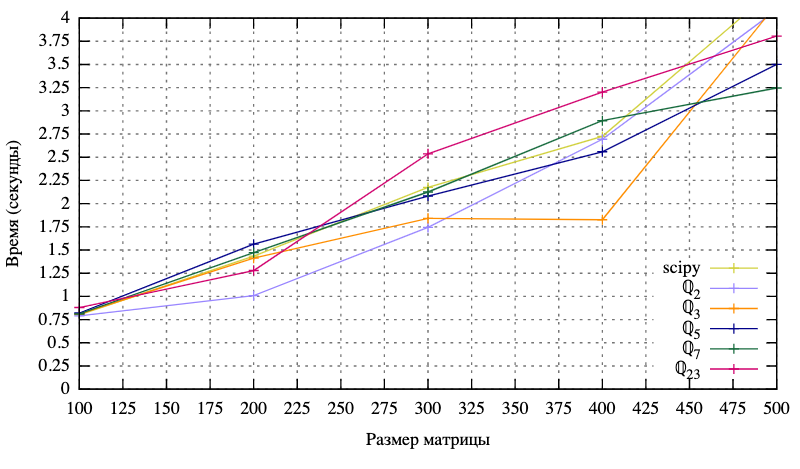
\includegraphics[width=0.85\linewidth]{../gnuplot/exp/plot.png}}
\caption{Сравнение классических и $p$-адических методов для вычисления матричной экспоненты.}
\label{img:exp:plot}
\end{figure}

Как видно из представленного графика \ref{img:exp:plot} - вычисление матричной экспоненты с помощью $p$-адических методов при использовании чисел из $\mathbb{Q}_2, \mathbb{Q}_3, \mathbb{Q}_5, \mathbb{Q}_7, \mathbb{Q}_{23}$ дают лучшие результаты, чем аналогичные классические методы из матиематического пакета |scipy| для ЯП Python.


\conclusion
В представленной магистерской выпускной квалификационной работе был разработан программный комплекс на ЯП Python для работы с наиболее распространенными объектами компьютерной алгебры, с использованием $p$-адической арифметики над полем рациональных чисел $\mathbb{Q}_p$. Представлены и описаны типы данных и алгоритмы работы с $p$-адическими числами как для однопоточного, так и для многопоточного случая. 

Тестирование программного комплекса было произведено на примере решения таких популярных прикладных задач как нахождение решения обыкновенного дифференциального уравнения, нахождение решения СЛАУ, вычисление собственных значений и векторов матрицы, а так же вычисление матричной экспоненты. Для всех тестов были произведены замеры производительности работы как однопоточного, так и многопоточного варианта вычислений, а также приведены графики, которые наглядно отображают полученные результаты. Тесты производительности многопоточной библиотеки показали, что что $p$-адическая арифметика дает хорошие результаты, а с учетом того, что не накапливает ошибку - даже лучшие, чем это могут сделать классические методы.

\bibliographystyle{biblio/ugost}
\bibliography{biblio/biblio}

\appendix

\section{Исходный код библиотеки для работы с $p$-адической арифметикой}

%Код приложения \verb"task.pl".
%\VerbatimInput[fontsize=\small, numbers=left, numbersep=2pt]{../python/setup.py}

% setup
\lstinputlisting[language=Python, numbers=left, showstringspaces=false, breaklines=true, basicstyle=\small, caption=Файл дистрибьюции библиотеки]{../python/setup.py}

% padic
\lstinputlisting[language=Python, numbers=left, showstringspaces=false, breaklines=true, basicstyle=\small, caption=Класс Padic]{../python/padic/padic.py}

% matrix
\lstinputlisting[language=Python, numbers=left, showstringspaces=false, breaklines=true, basicstyle=\small, caption=Класс Matrix]{../python/padic/matrix.py}

% determinant
\lstinputlisting[language=Python, numbers=left, showstringspaces=false, breaklines=true, basicstyle=\small, caption=Алгоритм вычисления определителя матрицы]{../python/algo/det.py}

% cramer
\lstinputlisting[language=Python, numbers=left, showstringspaces=false, breaklines=true, basicstyle=\small, caption=Метод Крамера]{../python/algo/cramer.py}

% Gauss
\lstinputlisting[language=Python, numbers=left, showstringspaces=false, breaklines=true, basicstyle=\small, caption=Метод Гаусса]{../python/algo/gauss.py}

% Jacoby
\lstinputlisting[language=Python, numbers=left, showstringspaces=false, breaklines=true, basicstyle=\small, caption=Метод Якоби]{../python/algo/jacoby.py}

% Euler
\lstinputlisting[language=Python, numbers=left, showstringspaces=false, breaklines=true, basicstyle=\small, caption=Метод Эйлера]{../python/algo/euler.py}

% R-K
\lstinputlisting[language=Python, numbers=left, showstringspaces=false, breaklines=true, basicstyle=\small, caption=Метод Рунге-Кутты]{../python/algo/rk.py}

% executor: ode
\lstinputlisting[language=Python, numbers=left, showstringspaces=false, breaklines=true, basicstyle=\small, caption=Функция для сравнения решения ОДУ]{../python/executors/ode.py}

% executor: sole
\lstinputlisting[language=Python, numbers=left, showstringspaces=false, breaklines=true, basicstyle=\small, caption=Функция для сравнения решения времени решения СЛАУ]{../python/executors/sole.py}

% generators: matrix
\lstinputlisting[language=Python, numbers=left, showstringspaces=false, breaklines=true, basicstyle=\small, caption=Генератор матрицы для тестов]{../python/generators/matrix.py}

\newpage
\section{Вспомогательные функции для метода Якоби}
\label{appendix:2}
\begin{algorithm}
\DontPrintSemicolon % Some LaTeX compilers require you to use \dontprintsemicolon instead
\KwIn{ $k$ }
\Begin {
	$m$ := $k+1$
	\For{$i \gets k+2$ \textbf{to} $n$} {
		\If{ \abs{S_{ki}} > \abs{S_{km}} } {
			$m := i$ 
		}
	}
	\Return m
}
\caption{функция $maxind$}
\end{algorithm}

\begin{algorithm}
\DontPrintSemicolon % Some LaTeX compilers require you to use \dontprintsemicolon instead
\KwIn{ $k, l, i, j$ }
\Begin {
$$
\begin{pmatrix}
  S_{kl} 
  S_{ij} 
\end{pmatrix}
:=
\begin{pmatrix}
  c & -s \\
  s & c
\end{pmatrix}
\cdot
\begin{pmatrix}
  S_{kl} 
  S_{ij} 
\end{pmatrix}
$$
}
\caption{процедура $rotate$}
\end{algorithm}

\begin{algorithm}

\DontPrintSemicolon % Some LaTeX compilers require you to use \dontprintsemicolon instead
\KwIn{ $k, t$ }
\Begin {
$y := e_k$ 
$e_k := y+t$
\If{$changed_k$ И ($y=e_k$)} {
	$changed_k$ := false
	state := state-1
}
\If {не $changed_k$) И ($y \neq e_k$)} {
	$changed_k$ := true
	state := state+1
}
}
\caption{функция $update$}
\end{algorithm}


\end{document}